\section{Parity violation, Helicity, and Chirality}
\subsection{Helicity/Chirality}
%%%%%%%%%%%%%%%%%%%%%%%%
 We need something in the theory of weak interaction that violates
 parity, and Wu's experiment suggests, that this element has something
 to do with helicity (see \figref{fig:WuInterpretation}. The magnetic field aligns (approximately) the nuclear spins. The $L$ value the \chem{Ni} nuclues is one unit less than that of the \chem{Co} nucleus. Angular momentum conservation (more precisely the conservation of $L_z + S_z$) forces the spins of the electron and the anti-neutrino to align with the spin of the \chem{Co}, and hence the magnetic field.
 If predominantly (or only?) helicity
 right-handed anti-neutrinos, and helicity left-handed electrons participate in the interaction, the anti-neutrinos go (predominantly) in the direction of the field (upwards) and the electron to go (predominantly) downwards.
 
 So, one idea could be to make
 a theory where only those participate, i.e. the weak interaction only
 applies to helicity left-handed particles and helicity right-handed
 antiparticles.

 This is only \emph{nearly} the answer.

 The reason this does not quite work is that helicity is not Lorentz
 invariant. What's one observer's left-handed (massive) particle is
 another observer's right-handed one. Just imagine you see a helicity
 left-handed particle passing by - and a train that's travelling faster
 than that particle. If you change frames by jumping on that train,
 you'll find that the spin of the particle remains the same, but the
 velocity flips, so the helicity is now right-handed.  But a decay
 that happens in one frame of reference must also happen in
 another.

 So helicity can't be the distinguishing factor, but seems to have
 something to do with it. And it would work for zero-mass particles,
 that travel with the speed of light - you can't over-take a particle
 that travels at the speed of light, therefore they have the same
 helicity in all frames.

 The solution to the problem is called chirality. Chirality is Lorentz
 invariant. It is defined such that it is equivalent to helicity for
 zero-mass particles (see table \ref{tab:helichi} for details), but
 different for massive particles.

 Strictly only chirality left-handed particles take part in the weak
 interaction. For massless particles, this corresponds to helicity
 left-handed matter particles and helicity right-handed antimatter
 particles.

 The probability that a massive particle with definite chirality, e.g. an electron
 emerging from a weak decay which is definitely chirality
 left-handed, is found in the 'wrong', or suppressed
 helicity state is
\begin{eqnarray}
\label{eq:wrongHeliProb}
\lefteqn{ \left|\braket{\mathrm{e^-\;right-handed\;helicity}}{\mathrm{e^-\;left-handed\;chirality}}\right|^2 } \nonumber\\
 &\approx &
 \half \left(1 - \beta \right)
 =
 \frac{m^2}{ 2E^2 \left( 1 + \frac{|\vec{p}|}{E}\right)}
  \sim \left\{
 \begin{array}{lr}
    \frac{m^2}{2E^2} &   |\vec{p}| \ll m \\
    \frac{m^2}{4 E^2} &  |\vec{p}| \gg m
  \end{array}
  \right\}
\end{eqnarray}
%%
\begin{table}
\caption{Helicity and Chirality for massless particles.  For massive
 particles with definite helicity, there is a
 contribution of the ``wrong'' chirality of the order of $\frac{m^2}{2E^2}$. This means for example that a helicity-right handed particle can still interact weakly, with a probability $\sim \frac{m^2}{2E^2}$, which goes to $0$ for $E\gg m$.
\label{tab:helichi}}
\begin{tabular}{c|cc c}
           &  chirality & helicity        & weak-interaction\\
           & \multicolumn{3}{|c|}{\small(for massless particle)} \\
 matter    &  left-handed & left-handed   &   yes \\
 matter    &  right-handed & right-handed &   no  \\
antimatter &  left-handed  & right-handed &   yes \\
antimatter &  right-handed & left-handed  &   no \\
\end{tabular}
\end{table}
%%
 For ultra-relativistic particles with $\beta \approx 1$ (implying $E\gg m^2$, i.e. relative to
 their energy, they are nearly massless), helicity and chirality are
 essentially equivalent. For particles at rest on the other hand, a
 chirality left-handed particle at rest has a 50\%-50\% probability of
 being helicity left-handed or right-handed (well, for a particle
 really at rest helicity is not so well defined, imagine a particle
 that's moving very very slowly).

 Under the operation \ps, both chirality and helicity change sign.

 So the \ps\ violation in the weak interaction is pretty massive - the
 formal sentence is \textbf{``parity is maximally violated in the weak
 interaction''}. A massless particle that is subject to the weak interaction is, after
 applying the parity operator, suddenly not subject to it anymore at
 all.
 %\footnote{For massive particles the situation is a little more complicated, as it turns out that massive particles cannot be, at the same time, mass eigenstates and chirality eigenstates - and since it's mass eigenstates what we consider physical "particles", massive particles are always an admixture of chirality left and righthanded, but this admixture can be very unbalanced.}

\subsection{Intermezzo: Fermi's Golden Rule for particle decays}
In the section after this, we will discuss the decay of the pion and find out how parity violation has a profound effect on it. 
\begin{figure}
\centering
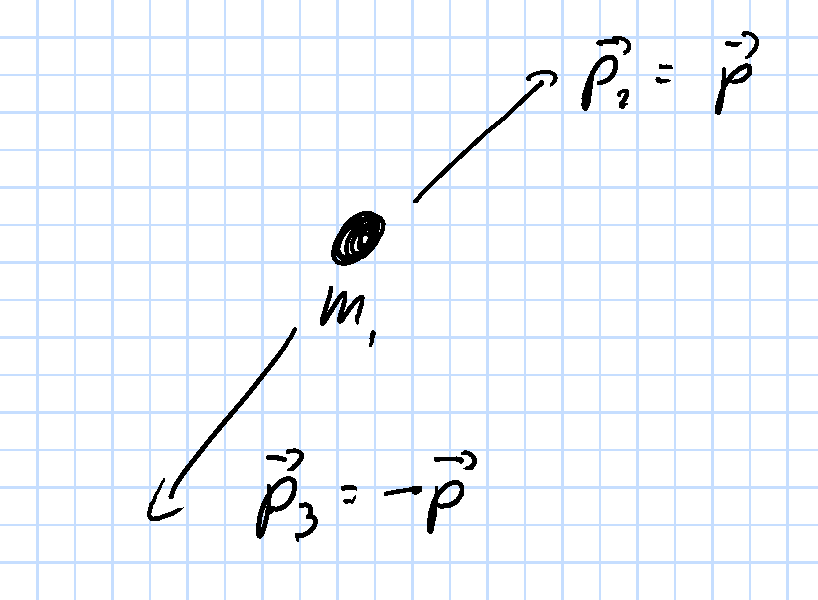
\includegraphics[width=0.4\textwidth]{fig/weak/Decay122}
\caption{Decay rate of particle $1$ into two particles (labelled $2$ and $3$) in the cm frame.\label{fig:Decay122}}
\end{figure}
Let's prepare ourselves by looking a bit closer at the "Golden Rule" that relates $\mathcal{M}_{fi}$ and hence the Feynman rules to decay rates, taking into account phase space density. (More on "Golden Rules" can be found in \appref{sec:GoldenRulesAndDensityOfStates}.)
\paragraph{Golden Rule for Decay Rates in cm frame}
(see \figref{fig:Decay122})
Decay of particle $1$ to particles $2, 3$ in the cm frame 
\begin{equation}
\Gamma_k = \frac{S}{8\pi} \frac{|\vec{p}|}{m_1^2} \left|\mathcal{M}_{fi}\right|^2
\end{equation}
Where $m_1$ is the mass of the decaying particle, and $\vec{p}$ is momentum of one of the daughter particles, $\vec{p} = \vec{p}_2 = -\vec{p_3}$. The subscript $k$ in $\Gamma_k$ indicates that this is the \emph{partial} width for the decay to this particular final state (that we label $k$). $S$ is $1$ when the final state particles are distinguishable (as in \prt{\pi^+ \to \mu^+ \nu_{\mu}}), except when the two final state particles are identical (as in \prt{\pi^0 \to \gamma \gamma}), in which case $S = \half$.
This is what you can do with the result of this calculation:
\begin{itemize}
\item $\Gamma_k$ is the partial width of the decay of particle $1$ to particles $2, 3$.
\item If I add up all partial widths (i.e. $\Gamma_k$ calculated for all possible final states $k$, added together) I get the total width $\Gamma = \sum_k \Gamma_k$. Its inverse is the average lifetime of the particle, $\tau = 1/\Gamma$. If I start with $N_0$ particles, I expect, after time $t$ (in the particles' restframe), to find $N(t) = N_0 e^{-\Gamma t}$.
\item If we have $N$ particles, the rate at which they will decay to this given final state is $N\Gamma_k$ (note that $N$ will decrease exponentially with time, $N(t) = N_0 e^{-\Gamma t}$).
\item If I observe $n$ decays of this given type of particle, the fraction of decays $n_k$ that I expect to find in final state $k$ is $n_k/n = \Gamma_k/\Gamma$. This ratio is called the Branching Fraction.
\end{itemize}
\paragraph{Phase Space Density}
Apart from some constants, the key factor that we find in addition to $\mathcal{M}_{fi}$ (which we get from Feynman rules) is the magnitude of the three-momentum of the daughter particles in the restframe of the mother, $|\vec{p}|$. This takes into account the number of different quantum mechanical states with (nearly [never forget Heisenberg's uncertainty principle]) the same momentum $|\vec{p}|$ that the final state can occupy - the decay rate is directly proportional to this. This proportionality factor is usually referred to as "phase space factor" or "phase space density". It is derived in \appref{sec:densityOfStates}. 
For the case of a decay of a particle with mass $M_A$ to two particles with masses $m_B, m_C$, the phase space factor is given by
\begin{equation}
 |\vec{p}| = \frac{\sqrt{(M_A^2 - (m_B + m_C)^2)(M_A^2 - (m_B - m_C)^2)}}{2M_A}
\end{equation}
Note that such a phase space factor applies no matter how the final state came about, by the decay of a particle, or through scattering. 
In the latter case, $M_A$ is replaced by the $cm$ energy. In either situation, when calculating ratios of rates, it only matters if the decay product are not much lighter than the mother particle / the collision energy. For $M_A \gg m_B, m_C$, this reduces to a constant ($\half M_A$) that cancels when calculating decay rate ratios. For example the phase space factor does not matter when calculating $R$ in \secref{sec:FormationOfJets}, because the collision energy is much higher than the masses of the quarks or leptons involved; it would also not matter when calculating ratios like $\Gamma(\prt{B^0 \to \pi^+ \pi^-})/\Gamma(\prt{B^0 \to K^+ K^-})$ because the $B^0$ meson is so much heavier than either pions or kaons. 
It will matter in the next section for the case where the pion decays to a muon and a neutrino. The muon's mass is very close to the pion's mass (this is why the muon, when it was discovered, was initially mistaken for the pion)\\
\fbox{\parbox{0.9\textwidth}{
\paragraph{We remember...}
\begin{itemize}
\item Fermi's Golden Rule relates Feynman rules and decay rates. Its key statement is:
$\Gamma_{f} \propto |\mathcal{M}_{fi}|^2 \times \mathsf{(phase-space-factor)}$.
\item The phase space factor takes into account the density of states and favours decays to lighter particles over decays to heavier particles.
\item When calculating ratios of rates with the same initial state, this phase space factor only matters if the mother particle's mass (or the collision energy) is not much higher than the masses of the decay products.
\end{itemize}
}}


\subsection{Pion decay} 
 Let us consider the ratio of decay rates of $\pi^- \to e^- \bar{v}_{e}$
 to $\pi^- \to \mu^- \bar{v}_{\mu}$. Naively, because of phase space
 considerations, one would expect the decay to the much lighter
 electron to dominate. However, the pion decays nearly always to the
 much heavier muon. Parity violation is the explanation.

 Due to angular momentum and momentum conservation, the two decay
 products of the $\pi$, which has spin 0, must have the same
 helicity. Assuming that the anti-neutrino is massless, and looking at
 table \ref{tab:helichi}, the anti-neutrino must have positive
 helicity. That leaves the electron or muon no choice but have
 positive helicity as well. But of course the electron/muon must also
 have negative chirality. From the previous section we know that the
 heavier the particle is, relative to its momentum, the more likely it
 is to have negative chirality and at the same time positive helicity.

\begin{figure}
\centering
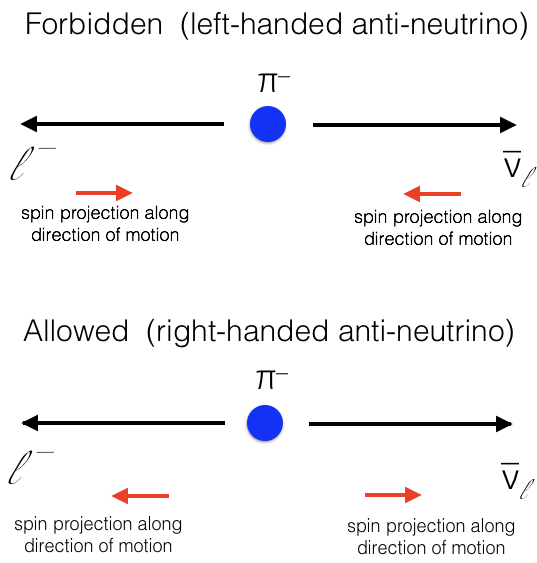
\includegraphics[width=0.6\textwidth]{fig/0_pionDecay}
\caption[Pion Decay]{Pion Decay: To conserve $\vec{L} + \vec{S}$, the spin-projections for the charged lepton ($\ell^-$) and the anti-neutrino have to be opposite, leading the the two possible configurations shown above. Since the neutrino is (nearly) massless, only the helicity right-handed anti-neutrinos interact, while helicity left-handed anti-neutrinos do not.
\label{fig:my_label}}
\end{figure}

 Actually, from \label{eq:wrongHeliProb} we can estimate the ratio of
 decay rates, neglecting phase-space effects. Let's start with the
 decay to electrons: Compared to the pion, both the electron and the
 neutrino are very light, and they'll share the energy of the decay
 approximately equally. The energy of the electron in the pion
 restframe is $\sim \half m_{\pi}$, so the probability of it
 interacting with the suppressed helicity is
\begin{equation}
 \sim \frac{m_e^2}{4 \cdot \half m_{\pi}^2}
 = \frac{m_e^2}{2 m_{\pi}^2}
\end{equation}
 Now the muon has nearly the same mass as the pion, and hence will
 stay (nearly) at rest in the pion restframe, while the neutrino
 carries off the energy of the decay, so $E_{\mu} \sim m_{\mu}$. So
 the probability for it to have the suppressed helicity is
\begin{equation}
 \sim \frac{m_{\mu}^2}{2 m_{\mu}^2} = \half
\end{equation}
 and the ratio between the two:
\begin{equation}
 \sim \frac{m_e^2}{m_{\pi}^2} \sim 1.3\cdot 10^{-5},
\end{equation}
 massively favouring the decay to the muon.
 On the other hand, the phase space factor
 \begin{equation}
 \Phi \propto |\vec{p}| = 
 \frac{m^2_{\pi} - m^2_{\ell}}{2 m_{\pi}}
 \end{equation}
(where $\ell$ is either the electron or the muon) favours the decay to the electron. Combining the two competing contributions gives an estimate of the decay rate ratio of
 \begin{equation}
 \frac{\Gamma(\pim \to e^- \overline{\nu}_e)}{
    \Gamma(\pim \to \mu^- \overline{\nu}_{\mu})}
\sim
 \frac{m_e^2}{m_{\pi}^2} 
    \left(
     \frac{m^2_{\pi} - m^2_{e}}{
     m^2_{\pi} - m^2_{\mu}}
    \right)
 \sim 0.4\cdot 10^{-4}
\end{equation}


 The full calculation can be found in many text
 books and leads to an additional factor of 
 $\left(
     \frac{m^2_{\pi} - m^2_{e}}{
     m^2_{\pi} - m^2_{\mu}}
    \right)$. 
The result is
\begin{equation}
 \frac{\Gamma(\pi \to e \nu_e)}{\Gamma(\pi \to \mu \nu_{\mu})}
=
\frac{m_e^2}{m_{\mu}^2} \left(\frac{m^2_{\pi} - m^2_{e}}{m^2_{\pi} -
  m^2_{\mu}}\right)^2
= 1.23 \cdot 10^{-4}.
\end{equation}
which is pretty close to our estimate.
So, due to the \ps-violation-induced \emph{helicity suppression}, the pion decay to the muon completely dominates over the decay mode to the electron (and in fact anything else, so charged pions essentially always decay to muons and (anti) muon neutrinos). This is the opposite of what one would expect without helicity suppression, where the electron mode would dominate because of phase space considerations. This result is in excellent agreement with the experimental value for the decay rate ratio of $(1.230\pm 0.004) \cdot
 10^{-4}$. 
A rather striking effect of \ps\ violation.

\section{\cs{}harge Conjugation}
\label{sec:ChargeConjugation}
 The Charge conjugation operator transforms particles to
 antiparticles. Like for the parity operator, it follows from $\cs^2=1$
 that it can have the eigenvalues $+1$ and $-1$.

 It is called 'charge conjugation' because it swaps all charges -
 positive and negative electric charge as well as colour charge (for
 the strong interaction) and weak charge. \cs\ also swaps the
 chirality quantum number (but not the helicity quantum number, but as
 you can see from table \ref{tab:helichi}, as far as the weak
 interaction is concerned, the effect is the same).

 Neutral particles can be (but don't have to be) \cs\
 eigenstates. Charged particles of course cannot. However,
 particle-antiparticle pairs of charged (or neutral) particles can
 also be \cs\ eigenstates (they might even have been created in the
 decay of a \cs\ eigenstate).

 Like \ps, \cs is a multiplicative quantum number. For a system of
 particles with well-defined C-parity the total \cs\ eigenvalue is the
 intrinsic \cs\ eigenvalues of the particles involved. 

 If the particles involved are not themselves parity eigenstates, but
 particle-antiparticle pairs, the C-parity number is given by a factor
 that derives from the behaviour of the total wavefunction under the
 exchange of particles, and is therefore different for fermions pairs
 and for boson pairs. For a pair of bosons (like $\pi^+\pi^-$ or
 $\gamma, \gamma$), C parity is $(-1)^{L}$, where $L$ is the angular
 momentum of the pair. For pairs of spin-\half fermions (like $e^+,
 e^-$), the factor is $(-1)^{L+S}$, where $S$ is the total spin
 quantum number of the system.

 The quantum numbers of particles are usually given in the following
 format:
\begin{equation}
%
  J^{(PC)} \;\;\;= \;\;\;\mbox{Spin}^{(\mathrm{parity,\;\; \cs-eigenvalue})}
%
\end{equation}
 The $J^{(PC)}$ of some important particles are:\\
\begin{tabular}{|*{7}{c|}}
\hline
 $\gamma$ & $\pi^0$ & $\pi^{\pm}$ & $K^0$   & $K^{\pm}$ & p & n
\\\hline
 $1^{--}$ & $0^{-+}$& $0^{-}$     & $0^{-}$ & $0^{-}$   & $\half^{+}$
 & $\half^{+}$
\\
\hline
\end{tabular}

For a system of $C$-eigenstates:
\[
\prod\limits_{\mathsf{all\;particles}}
\mbox{(intrinsic C)}
\]
For a particle anti-particle pair of bosons that are not $C$
eigenstates (e.g. $\pi^+\pi^-$):
\[
C = (-1)^L
\]
This is a consequence of the fact that here, \cs has the same effect as \ps.
For a fermion-antifermion pair (e.g. $e^+ e^-$) it's a bit more complicated, we have to account for the behaviour of the wave function under spin exchange. For relative angular momentum $L$ and and total spin $S$:
\[
C = (-1)^{L+S}
\]



\section{\cp}
\label{sec:CPV_CP}
 \cp\ is simply the combined operation of \cs\ and \ps.
 For \cp\ eigenstates (only neutral particles can be \cp\ eigenstates, or
 systems of particles with overall zero charge), \cp\ is simply
 calculated by multiplying the $C$ and the $P$ quantum numbers.

 Applying the rules for \cs\ and \ps quantum numbers from the
 previous section this means for systems of particles:
\begin{itemize}
\item For a system of \cp\ eigenstates the total \cp\ number is given my
  multiplying the intrinsic \cp\ quantum numbers of the particles
  involved, times a factor $(-1)^L$.
\item A particle-antiparticle pair of bosons has the \cp\ eigenvalue
  $+1$, and a fermion-antifermion pair $(-1)^{S+1}$.
\end{itemize}


\subsection{Time Reversal and the \cpt\ theorem}
 The operation of time reversal reversed the direction of motion,
 i.e. it is as if you would run the movie backwards. The combined
 symmetry \cpt\ is believed to be a good symmetry of any sensible theory
 for rather fundamental reasons (I think it's causality and Lorentz
 invariance this is based on). \cpt\ violation would be big news,
 because it's certainly not expected.

 This means that one can usually consider \cp\ violation equivalent to
 \ts\ violation.

\section{Discovery of \cp\ violation}

 It is easy to see why, from what we have seen so far, \cp\ seems like a
 good candidate for good symmetry. We found that the requirement that
 only chirality left-handed particles participate in the weak
 interaction has the effect that helicity-left-handed particles
 and helicity-right-handed antiparticles take part. Parity
 transforms left and right handed helicity, and charge conjugation
 transforms particles to antiparticles, so under \cp\ we transform a
 helicity left-handed particle into a helicity right-handed
 antiparticle, so something that interacts weakly to something that
 still interacts weakly. Exactly in the same way? We'll see - in many
 cases yes, but in general, no.


 Originally it was hoped that \cp\ symmetry would replace the 'lost'
 \ps\ symmetry, and it came as a surprise when in 1964 Cronin and Fitch
 discovered that \cp\ was in fact violated in the neutral Kaon
 system\cite{cpdiscovery}.

 As opposed to the neutral pion, the neutral Kaon is not its own
 antiparticle. In fact the koans mix (see later) to form two distinct
 \cp\ eigenstates with well-defined (and different) mass and lifetime (at least in the absence of \cp\ violation):
 \begin{align}
 \label{eq:KaonCPevenOdd}
  \ket{K^0_{\mathsf{CP-even}}} &= \frac{1}{\sqrt{2}}\left(\ket{K^0} + \ket{\overline{K}^0}\right)
   &
  \ket{K^0_{\mathsf{CP-odd}}} &= \frac{1}{\sqrt{2}}\left(\ket{K^0} - \ket{\overline{K}^0}  \right)
 \end{align}
 The \cp\ even state decays into two pions (that's how we know it's \cp\ even) while the \cp\ odd state has to decay to three pions to conserve \cp\, meaning far less phase space and a longer lifetime.
 These states are therefore referred to as "K-short", \prt{K_S^0}, 
 and "K-long", \prt{K_L^0}.

 In 1964, Cronin and Fitch discovered that the supposedly \cp\-odd
 \prt{K_L} sometimes decays to two pions, and thus \cp\ is violated
 \ref{cpdiscovery}. 
 It means that the mass eigenstates (i.e. the eigenstates of the Hamiltonian), 
 \prt{K_S^0} and \prt{K_L^0} 
 cannot anymore be identified with the \cp\ eigenstates in \eqnref{eq:KaonCPevenOdd}. 
 It means that in this sytem $[H,CP] \neq 0$, hence \cp\ is violated.

 Now we have two subjects to cover, which will finally lead us to B
 mesons and mixing. One is mixing of neutral particles (like neutral
 Kaons or B mesons). The other is also called mixing but refers to the
 quark-mixing matrix. This is important because this is where \cp\
 violation in the Standard model occurs. This is where we
 start.


\section{Quark Mixing and \cp\ violation}

 Now we finally connect the two seemingly disparate subjects we just
 treated, \cp\ violation and quark mixing.

 The logic is the following: \cp\ violation is observed in weak decays of
 quarks. Weak decays of quarks are governed by quark mixing. \cp\
 violation is due to quark mixing?

\subsection{Quark transitions under \cp\ and \ts}
 As we established above, the transition amplitudes of quarks are
 proportional to the relevant mixing matrix element. So, apart from a
 common factor, the matrix elements of the mixing matrix are the
 transition amplitudes of the quarks. It is convenient to write the
 mixing matrix in the following way:
\begin{equation}
 \vII{d^{\prime}}{s^{\prime}} =
 \mII{V_{ud}}{V_{us}}
     {V_{cd}}{V_{cs}}
 \vII{d}{s}
\end{equation}
  This is the same equation as before, just written in a different,
  convenient notation.

\paragraph{Down to Up transitions}
  With this notation, a $d\to u$ transition has an
  amplitude $V_{ud}$, a $s \to u$ transition an amplitude $V_{us}$,
  etc (all to be multiplied by a common factor that we will ignore).

\paragraph{Up to Down, or the effect of \ts}
  Transitions in the other direction (from u-type to down-type quarks)
  have the complex-conjugate amplitude, so $u\to d$ has the amplitude
  $V^{*}_{ud}$ and $c\to d$ has the amplitude
  $V^{*}_{cd}$, etc. Note that this is not true for amplitudes in
  general, but it is for mixing matrix elements. This result does not
  follow from what we have done in the preceding section, and a
  derivation would be beyond the scope of this lecture, so we just
  state it.

\paragraph{The effect of \cp}
  \cp\ conjugation is equivalent to complex-conjugating the mixing
  matrix element, so $\bar{d} \to \bar{u}$ transitions have amplitude
  $V^{*}_{ud}$, etc. Again, we just state this result w/o any further
  justification, except for mentioning that we could have guessed this
  from \cpt\ symmetry and the previous paragraph. Note that this is
  for \cp\ conjugation - \cs\ conjugation alone would have a different
  effect, the transition amplitude would be zero (it is weak
  interaction after all), it must be \cp. Here we assume that we are
  dealing always with chirality left-handed quarks.

Hence...
\textbf{To put \cp\ violation in mixing we need complex mixing matrix
  elements.}

\fbox{\parbox{0.98\textwidth}{\label{box:CKMVertices}
    \textbf{Associating quark mixing (CKM) matrix elements to vertices in Feynman diagrams:\\}
    \begin{tabular}{cccc}
    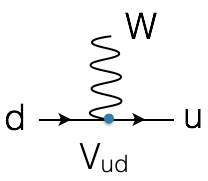
\includegraphics[width=0.18\textwidth]{fig/C_P_CP/Vud_d2u}
    &
    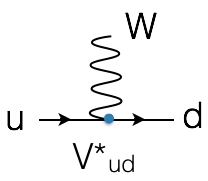
\includegraphics[width=0.18\textwidth]{fig/C_P_CP/Vud_u2d}
    &
    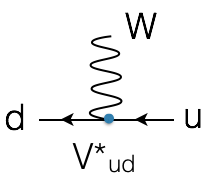
\includegraphics[width=0.18\textwidth]{fig/C_P_CP/Vud_antid2u}
    &
    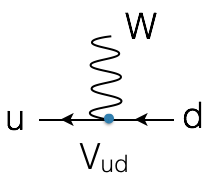
\includegraphics[width=0.18\textwidth]{fig/C_P_CP/Vud_antiu2d}
    \end{tabular}\\
    In the above example you can replace $d$ with any down-type quark (i.e. $s, b$) and $u$ with any up-type quark (i.e. $c, t$). E.g.:\\ 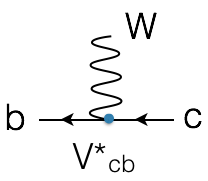
\includegraphics[width=0.18\textwidth]{fig/C_P_CP/Vcb_antib2c}.
}}

\subsection{A closer look at mixing}
 Now so far, our Cabibbo mixing matrix only has real elements. Maybe
 one of them is in fact complex, thus explaining the observed \cp\
 violation in the Kaon system?

 Let us first look at the constraints that exist on the Cabibbo
 matrix. We view it as a basis transformation, transforming the mass
 eigenstates ($d,s$) to the weak-interaction partners of the $u$ and
 the $c$ quark, $d^{\prime}, s^{\prime}$. For such a
 transformation, we demand that the length of the state vector does
 not change - i.e. we don't get more quarks, for fewer, after the
 transformation than before.
 Mathematically this means:
\begin{eqnarray}
 \vII{d^{\prime}}{s^{\prime}}^{\dagger}
 \vII{d^{\prime}}{s^{\prime}}
=
 \left( V \vII{d}{s}\right)^{\dagger}
  V \vII{d}{s}
&=&
 \vII{d}{s}^{\dagger}
 V^{\dagger} V
 \vII{d}{s}
\nonumber\\
&=&
 \vII{d}{s}^{\dagger}
 \vII{d}{s}
\end{eqnarray}
 where $\dagger$ stands for ``Hermitian conjugate'', i.e. transposed
 and then complex-conjugated.  Since the above expression must be true
 for any $d,s$ vector, this implies for the mixing matrix $V$:
\begin{equation}
 V^{\dagger} V = 1
\end{equation}
 In words: \textbf{$V$ must be a unitary matrix}. In fact, this is all
 that theory predicts about $V$.

\subsubsection{Phases in a $2\times 2$ mixing matrix}
 A general $2\times2$ unitary matrix can be parameterised by one
 (real) angle, and three complex phases. Now that looks like good news
 - complex phases is what we wanted. But not all complex phases are
 physically meaningful, as we know from basic quantum mechanics. If we
 remove all 'arbitrary' phases, and still are left with a complex
 phase in the mixing matrix, then we actually have a complex mixing
 matrix element where the fact that $V_{ij}^* \neq V_{ij}$ under \cp\
 actually has measurable consequences.

 So what are those arbitrary phases? Essentially each phase in the
 definition of a quark wave function. Now in the entire theory, this
 sort of thing can only be done once - once you've made use if this
 freedom to define the phases of the quark wavefunction, you can't do
 it again. But, take it on trust, no-where else in the Standard Model
 has this freedom yet been exploited, so we can do it here.

 Since the elements of the mixing matrix only appear sandwiched
 between quark wave functions, we can re-define the phases of those
 quark wave functions to remove phases from the mixing matrix.

 There is one phase for each quark field. One of them can be removed
 without having an effect, by removing one over-all phase. This
 over-all phase does not affect the mixing matrix because the
 mathematical expressions in which the mixing matrix appears when we
 calculate transition amplitudes are of the form $u^* V d$, i.e. one
 quark function always enters as the complex conjugate (as usual, in
 matrix elements). If you add an over-all phase to the d and the $u$,
 it'll get cancelled in the expression above since it enters with the
 opposite sign in the $u^*$. It is the old thing that phase
 differences matter, but not the overall phase. What matters are the
 relative phases of the quarks, and of those we have $3$ for a theory
 with 4 quarks, or more generally:

 \textbf{For $n$ quarks we can remove $n-1$ phases from the mixing
 matrix} by fixing the otherwise arbitrary relative quark phases.

 We only had three complex phases in our $2\times 2$ unitary matrix in
 the first place, so we can remove all complex phases of the quark
 mixing matrix, and our mixing matrix is real and determined by one
 parameter - the one we already know, the Cabibbo angle. To summarise
 the important result of this section:

\textbf{For two generations of quarks, there is no room for \cp\
 violation in quark mixing.}

\section{CKM and 3 Generations}

 While everyone realised that \cp\ violation could not be accommodated
 in 2-generation quark mixing, it was M. Kobayashi T. Maskawa who
 realised that this could imply that there are in fact 3 generations
 \cite{progtp.km}.

 Let us do the same counting exercise again that we did above, but now
 for 3 generations, 6 quarks. Now we have a $3\times 3$ unitary
 matrix. This has 9 complex entries, i.e.~18 parameters. The unitarity
 condition provides 9 constraints, leaves 9 free parameters for a
 generic unitary $3\times 3$ matrix. These can be taken as three real
 angles (e.g. Euler angles parameterising real rotations), plus 6
 complex phases.

 With three generations of quarks we have 6 quarks, so we can
 re-define $6-1=5$ relative quark phases to remove complex phases from
 the mixing matrix.
%
 This leaves us with one irremovable, meaningful complex phase. We have
 no prediction for its value, but it \emph{could} parametrise \cp\
 violation. 
%
 Note that, with this, Kobayashi and Maskawa predict the existence of
 an entire generation of new particles (at least 2 quarks, and then
 presumably, for symmetry, 2 leptons) from the observation of \cp\
 violation in Kaon decays, which involve Kaons and pions, made from
 $u,d,s$ quarks, i.e. quarks from only 2-generations.

 All of the predicted particles were subsequently found. The new
 quarks are the bottom quark, discovered in 1977
 \cite{beautydiscovery}, and the very heavy top quark, discovered in
 1994 \cite{topdiscovery}.

 But the real test of the KM theory is not just the existence of a
 third generation, but that \textbf{\cp\ violation is parametrised by
 a single complex phase} in the quark mixing matrix. The $3\times 3$
 quark mixing matrix is called the CKM matrix, after Cabibbo,
 Kobayashi and Maskawa.

 Our quarks are:
\begin{equation}
\vII{u}{d^{\prime}},\;\; \vII{c}{s^{\prime}},\;\; \vII{t}{b^{\prime}}
\end{equation}
 with
\begin{equation}
\vIII{d^{\prime}}{s^{\prime}}{b^{\prime}} = V_{CKM}\vIII{d}{s}{b}
\end{equation}

% And the CKM matrix can be parametrised as
%\begin{equation}
%\label{eq:th.b.vckmpara.pdg}
%V_{\mathrm{CKM}}=
%\mIII{ c_{12}c_{13}    }{
%                    s_{12}c_{13}       }{
%                                  s_{13}e^{-i\delta_{13}} }{
%     -s_{12}c_{23}-c_{12}s_{23}s_{13} e^{i \delta_{13}} }{
%             c_{12}c_{23}-s_{12}s_{23}s_{13}e^{i \delta_{13}} }{
%                     s_{23}c_{13}}{
%     s_{12}s_{23}-c_{12}c_{23}s_{13}e^{i \delta_{13}}}{
%             -c_{12}s_{23}-s_{12}c_{23}s_{13}e^{i \delta_{13}}}{
%                     c_{23}c_{13} }
%\end{equation}\\
% with the three real angles $\theta_{12}, \theta_{13}, \theta_{23}$
% and the complex phase $\delta_{13}$, were we used the short-hand
% notation $c_{ij}=\cos{\theta_{ij}}$ and
% $s_{ij}=\sin{\theta_{ij}}$ for $i,j=(1,2), (1,3), (2,3)$ to fit it
% all in.

\section{The structure of the CKM matrix}
 Let us label the elements of the CKM matrix in a way analogous to the
 Cabibbo matrix earlier:
\begin{equation}
\label{eq:th.b.ckmlabel}
V_{\mathrm{CKM}}=\mIII{ V_{ud} }{ V_{us} }{ V_{ub} }{
                        V_{cd} }{ V_{cs} }{ V_{cb} }{
                        V_{td} }{ V_{ts} }{ V_{tb} }
.
\end{equation}
 Then the transition amplitude from a \qrk{d} to a \qrk{u} quark is
 proportional to $V_{ud}$, the transition amplitude from a \qrk{u} to
 a \qrk{d} quark to $V_{ud}^{\ast}$, etc.

 Experimentally, it is found that the magnitudes of the CKM matrix
 elements follow a clear structure. In terms of the sine of the
 Cabibbo angle, $\lambda\equiv \sin\theta_C=0.22$, the CKM matrix is (very) approximately:
\begin{equation}
\label{eq:ckmLambda}
\mIII{ 1 }{\lambda}{\lambda^3 e^{-i\gamma}}{
      -\lambda}{1}{\lambda^2}{
      \lambda^3 e^{-i\beta}}{-\lambda^2}{1}
.
\end{equation}\\
 Note that this striking structure is not predicted by the Standard
 Model - it is however allowed.  This observation led Wolfenstein to a
 parametrisation of the CKM matrix as a power series in the parameter
 $\lambda$, which is, up to \order{\lambda^3}, given by
 \cite{wolfenstein}: {\small
\begin{equation}
\mIII{ 1-\half \lambda^2    }{ 
                   \lambda                }{ 
                        A\lambda^3\left(\rho-i\eta\right) }{
       -\lambda             }{ 
                    1-\half \lambda^2     }{ 
                        A \lambda^2                        }{
      A\lambda^3\left(1-\rho-i\eta\right)}{
                    -A \lambda^2      }{
                        1                                  }
.
\end{equation}}\\
 where $A, \rho, \eta$ are real parameters of order $1$. The \cp\
 violating phase is parametrised by $\eta$. Up to \order{\lambda^3},
 the only complex elements in this parametrisation are $V_{td}=|V_{td}|e^{-i\beta}$ and
 $V_{ub}=|V_{ub}|e^{-i\gamma}$, where $\gamma \approx 68^o$ and $\beta = 21^o$ (if you include higher order terms, additional CKM matrix element acquire - small - complex phases).
 Putting in some measured values:
 \begin{equation}
\label{eq:th.b.ckmlabel_1}
  V_{\mathrm{CKM}}=\mIII{ V_{ud} }{ V_{us} }{ V_{ub} }{
                        V_{cd} }{ V_{cs} }{ V_{cb} }{
                        V_{td} }{ V_{ts} }{ V_{tb} }
\approx
                 \mIII{ 0.97 }{ 0.23 }{ 0.0037\cdot e^{-i \gamma} }{
                        -0.23 }{ 0.97}{0.041 }{
                        0.0087\cdot e^{-i \beta} }{-0.041 }{0.9991 }
\end{equation}
where $\gamma \approx 68^o$ and $\beta = 21^o$. Don't worry about all the different version of the CKM matrix given here. It is this last version that we will use (and that's given in the formula sheet). But have a look at the others, it helps appreciate the rather striking (near diagonal) structure of the matrix.

 
\subsection{Why \cp\ violation in the Kaon system is small}
 
 From the preceding chapter we understand why \cp\ violation in the
 Kaon system must be a small effect. Kaon decays involve, to first
 order, only two generations of quarks: $(u,d)$ and $(c,s)$. We just
 established that a $2\times 2$ mixing matrix does not contain \cp\
 violating terms. Now this is not the complete story, it is a bit more
 complicated: In the presence of three generations, we would have
 to revise our argument for the $2\times 2$ sub-matrix a little bit,
 after all now the $3\times 3$ matrix is unitary, so the unitarity
 constraints that we used in our complex-phase counting exercise
 don't apply to the $2\times 2$ sub-matrix anymore.

 But looking at the structure of the CKM matrix (Eq
 \ref{eq:ckmLambda}), we also see that the two first generations
 couple only very weakly to the third, in which case the $2\times 2$
 sub-matrix does in fact, to first order, represent a stand-alone
 $2\times 2$, unitary mixing matrix, without (meaningful) complex
 phases, and hence w/o \cp\ violation. In terms of the Wolfenstein
 parameterisations, it turns out that even up to $4th$ order in the
 small parameter $\lambda=0.22$, the top-left $2\times 2$ block is
 real.

 Therefore, \cp\ violation in the Kaon system could only be a higher
 order phenomenon, induced by the highly suppressed interaction of the
 first two generations with the third. We were probably very lucky to
 see it as early as we did. Because the mass of the neutral Kaon is very close the the
 mass of the three pions that the \cp-odd Kaon decays to, this decay is
 very much dis-favoured by phase-space - but very much favoured by the
 approximate \cp\ conservation. This phase-space suppression is the reason
 why the $K_L$ (``K-long'') lives so long. Relative to that, the decay
 to two pions is much favoured by phase space, which is why the $K_s$
 ``K-short'' lives so short relative to the $K_L$. Without this
 coincidence, where phase-space highly favours the 'forbidden' decay,
 we might never have seen the \cp\-violating decay of $K_L\to \pi\pi$ at
 all, or most likely much later.

\subsection{Where to look for \cp\ violation}
 Looking at the CKM matrix, we see that the only potentially large
 complex phases are in the top right corner and the bottom left. We
 therefore want decays that involve $b\to u$ transitions or $t\to d$
 transitions. First of all, and this doesn't surprise us after the
 preceding discussion, this means we want decays of quarks from the
 third generation.

 Clearly, $b \to u$ transitions we get from decays of $B$-hadrons,
 which is the generic terms for hadrons involving $b$
 quarks. Interestingly, $t \to d$ transitions are also accessible in a
 certain, rather common species of B hadrons, the \Bdo\ mesons. Where
 and how will be discussed later in the section on B mixing.


\subsection{Unitarity Triangles*}
\label{sec:th.b.triangles}
The requirement that the CKM matrix is unitary:
\begin{equation}
\Vckm \Vckm^{\dagger} = \mathbf{1}
\end{equation}\\
 leads to 9 conditions, which are automatically fulfilled in any
 of the above parameterisations. Six of them can be expressed in
 so-called unitarity triangles, which are three complex numbers adding
 up to zero displayed in the complex plane. Below, the six unitarity
 relations leading to the six triangles are listed, together with an
 indication of the length of each side in orders of $\lambda$: {\small
\begin{equation}
\label{eq:CKMUnitarity}
\begin{array}{l c c c c c c c}
1)&V_{ud}^{\ast}V_{us}&+&V_{cd}^{\ast}V_{cs}&+&V_{td}^{\ast}V_{ts}&=&0\\
  & \order{\lambda}   & &\order{\lambda}    & & \order{\lambda^5} & & \\
  &                   & &                   & &                   & & \\
2)&V_{cd}^{\ast}V_{ud}&+&V_{cs}^{\ast}V_{us}&+&V_{cb}^{\ast}V_{ub}&=&0\\
  & \order{\lambda}   & &\order{\lambda}    & & \order{\lambda^5} & & \\
  &                   & &                   & &                   & & \\
3)&V_{us}^{\ast}V_{ub}&+&V_{cs}^{\ast}V_{cb}&+&V_{ts}^{\ast}V_{tb}&=&0\\
  & \order{\lambda^4} & &\order{\lambda^2}  & & \order{\lambda^2} & & \\
  &                   & &                   & &                   & & \\
4)&V_{cd}^{\ast}V_{td}&+&V_{cs}^{\ast}V_{ts}&+&V_{cb}^{\ast}V_{tb}&=&0\\
  & \order{\lambda^4} & &\order{\lambda^2}  & & \order{\lambda^2} & & \\
  &                   & &                   & &                   & & \\
5)&V_{ud}^{\ast}V_{td}&+&V_{us}^{\ast}V_{ts}&+&V_{ub}^{\ast}V_{tb}&=&0\\
  & \order{\lambda^3} & &\order{\lambda^3}  & & \order{\lambda^3} & & \\
  &                   & &                   & &                   & & \\
6)&V_{ub}^{\ast}V_{ud}&+&V_{cb}^{\ast}V_{cd}&+&V_{tb}^{\ast}V_{td}&=&0\\
  & \order{\lambda^3} & &\order{\lambda^3}  & & \order{\lambda^3} & & \\
  &                   & &                   & &                   & & \\
\end{array}
\end{equation}}\\
 If there is no \cp\ violation, the triangles all degenerate to
 lines. Describing \cp\ violation in terms of unitarity triangles has
 the advantage that changing the parametrisation of the CKM matrix,
 and hence the phase-convention for the quarks, simply rotates the
 whole triangle in the complex plane, but leaves the side lengths and
 the relative angles inside the triangle unchanged. Therefore the
 unitarity triangles are a convention--independent way of parameterising
 \cp\ violation in the \sm.

 The area of the all unitarity triangles is the same and is the
 geometric, convention-independent equivalent of the single complex
 phase in the CKM matrix \cite{Jarlskog:triangle_area}:
\begin{equation}
\mbox{Area of all triangles} = \half \left|J\right|
\end{equation}\\
with
\begin{equation}
J=\sum_{m,n=1}^3 \epsilon_{ikm}\epsilon_{jln} 
  \Imag\!\left( V_{ij} V_{kl} V_{il}^* V_{kj}^* \right)
\end{equation}
\begin{displaymath}
\mbox{ for any } i,j,k,l \in \left\{1,2,3\right\}
\end{displaymath}

\subsection{\emph{The} Unitarity Triangle and the Angles \gam, \bet}
\label{sec:th.b.thetriangle}
 Most of the triangles have very unequal sides. To measure \cp\
 violation in decays related to such triangles, for example in the
 \prt{K^0} system associated to triangle number 1, is very difficult:
 the two long sides have little relative phase difference and
 therefore little \cp\ violating effects; the third short side might have a
 large phase difference relative to the long sides, but this angle is
 then not very well constrained anymore by the length of the other
 sides - a small error on one of the long sides corresponds to a
 relatively large error on the angle ($\propto 1/\mbox{(length of
 short side)}$), and the most appealing feature of the unitarity
 triangles is in fact that it relates \cp\ violating phases to other
 measurements in quark decays and thus tests the SM model.


 Only in the last two triangles are all sides of the same order of
 magnitude. Both are related to observables in decays of neutral \prt{B}
 mesons: number $5$ to \Bso\ decays and number $6$ to \Bdo\ decays. Up
 to \order{\lambda^3} in the Wolfenstein parametrisation, the two
 triangles coincide. Therefore triangle number 6 is called \emph{The}
 Unitary Triangle.
\begin{figure}
\caption{\emph{The} Unitary Triangle\label{fig:th.b.triangle}}
\setlength{\unitlength}{1.2cm}
\begin{picture}(7,2.2)

\put(6,0){\vector(-1,0){5}}
\put(1,0){\vector(1,1){2}}
\put(3,2){\vector(3,-2){3}}

%\put(3,1.5){\mbox{$\alpha$}}
\put(1.5,0.15){\mbox{$\gamma$}}
\put(5,0.15){\mbox{$\beta$}}

\put(5,1){\mbox{$V_{tb}^{\ast} V_{td}$}}
\put(0.3,1){\mbox{$V_{ub}^{\ast} V_{ud}$}}
\put(3,0.15){\mbox{$V_{cb}^{\ast} V_{cd}$}}
\end{picture}
\end{figure}
 This is shown in figure \ref{fig:th.b.triangle}, where also the
 angles \gam\ and \bet\ are defined. The angles \bet\ and \gam\ are the complex phases of the only complex CKM matrix elements (up to $\order{\lambda^3}$, $V_{td}=|V_{td}|e^{-i\beta}$ and $V_{ub} = |V_{ub}|e^{-i\gamma}$. The parameter $\alpha$ that is
 often found in the literature, corresponds to the third angle in figure
 \ref{fig:th.b.triangle}; $\alpha \equiv \pi-\bet-\gam$ (but there is no CKM element with phase $\alpha$. Because \order{\lambda^3}, \bet\ and
 \gam\ are the only non-zero phases in the CKM matrix, and only decays
 involving \qrk{b \to u} or \qrk{d \to t} transitions can violate \cp.
 Both are accessible in the \Bdo\ system, $\gamma$ and other
 interesting parameters are also accessible in the \Bso\ system.

 The unitarity triangle is a convenient way to relate \cp\ violation
 measurements to other measurements in the Standard Model. Non
 \cp-violating measurements of quark transition rates measure the
 absolute size of CKM elements, and hence the length of the sides of
 the triangle. \cp\ violation measurement measure the angles.

 Any inconsistency in these measurements would indicate a failure of
 the Standard model and be a much sought-after hint of new physics.

\subsection{Summary: \cp\ Violation in the Standard Model}
 \begin{itemize}
 \item In the Standard Model, \cp\ violation is parametrised by a
 single complex phase in the CKM matrix. The SM is therefore very
 predictive wrt \cp\ violation.
 \item There are two elements in the CKM matrix with large complex
 phases, these are $\beta$ and $\gamma$ and both depend on the
 previously mentioned single phase. Both are accessible in the B
 system.
 \item The SM predicts that the CKM matrix is unitary.
 \item The Unitarity triangle relates CP-violating phases to other
 measurements, for example absolute transition rates that measure the
 lengths of the side of the unitarity triangle. Any inconsistency
 would indicate new physics.
\end{itemize}

\section{Neutral Meson Mixing/Oscillations}
A phenomenon that is not in itself \cp\ violating, but that is, as we will see in \secref{sec:CPVinB}, closely related, is the phenomenon of meson anti-meson mixing. It is the fascinating property of neutral Kaons ($\overline{s}d$), neutral D-mesons ($c\overline{u}$) and neutral B mesons ($\overline{b}d$) to turn into their own antiparticles and back. This phenomenon is also called "oscillation" because the Meson oscillates between two states, one of which is the antiparticle of the other.\\
\exercise{
Quick question: Why do \piz\ mesons not oscillate?\\
\rotatebox{180}{Because they are their own antiparticle}
}\\

\subsection{Meson mixing in the absence of \cp\ violation}
The discussion below will be applicable to any neutral meson system, we'll use the \Bo, \Bob\ system as an example.

\subsubsection{The two-states \Se\ for the neutral meson system*}
\label{sec:details}
The \Se\ for a superposition of flavour eigenstates, $ a \ket{\Bo} + b
\ket{\Bob}$, is:
\begin{equation}
\label{eq:th.a.se}
%
i\dbyd{}{t}\vII{a}{b}= \op{H} \vII{a}{b}.
%
\end{equation}\\
 

 It can be shown that \cpt\ invariance implies that the diagonal elements of \op{H} are the same and \op{H} and therefore be written as:
\begin{equation}
\op{H}=\mII{h_{11}}{h_{12}}{h_{21}}{h_{11}}.
\end{equation}
The crucial bit are the off-diagonal elements. They make matrix elements like this $\bra{\Bo}
\op{H}\ket{\Bob}$ non-zero, so they allow $\Bo\ \to \Bob$ transitions. If we were dealing with charged particles (like \Bp, \Bm), clearly such transitions would not be allowed, and the Hamiltonian would be diagonal. But for neutral mesons like \Bo, \Bob, as well as \Ko, \Kob, and \Do, \Dob, no conservation law is violated in such transitions, and the off-diagonal elements are non zero. You will see a Feynman diagram for such a transition later in the notes. As we will show below, these off-diagonal elements lead to two distinct mass eigenstates with different masses.

 \op{H} has the following eigenvalues:
\begin{equation}
\lambda_{H,L}=h_{11}\pm \sqrt{h_{21}\cdot h_{12}}
\end{equation}
The diagonalised Hamiltonian is:
\begin{eqnarray}
%
\lefteqn{\op{H_d} = \mII{H_H}{0}{0}{H_L} }\nonumber\\
         & &
= \mII{h_{11} + \sqrt{h_{12} h_{21}}\!\!\!}{0}
    {0}{\!\!\!h_{11} - \sqrt{h_{12} h_{21}}}
.
\nonumber\\
\mbox{}
\end{eqnarray}
 The eigenstates of the Hamiltonian (i.e. what we'd call "real" or "physical" particles), are given by:
\begin{equation}
\label{eq:th.a.def_Bl_Bh}
\ket{\prt{B_{H,L}}} = p \ket{\Bo} \mp q \ket{\Bob},
\end{equation}
with $|p|^2 + |q|^2 = 1$ and
\begin{equation}
\frac{q}{p}= -\sqrt{\frac{h_{21}}{h_{12}}}.
\end{equation}\\
The indices $H$ and $L$ stand for "heavy" and "light" mass eigenstate.
 The diagonalised Hamiltonian \op{H_d} is:
 
\op{H} can be written in terms of two Hermitian matrices, \op{M}, and \op{\Gamma}, as
\begin{equation}
\op{H}= \op{M} + \frac{i}{2} \op{\Gamma}
\end{equation}
where \op{M} represents the energy (mass) of the particles, and \op{\Gamma} represents their decay.
(If the particles were stable, \op{\Gamma} would be zero and the Hamiltonian would be Hermitian as one might expect, but since they do decay, we do not represent the full set of available states with \Bo, \Bob, hence the Hamiltonian is not Hermitian, as probability is not conserved - the system can leave our subspace. This is represented by \op{\Gamma}).

The diagonal mass and decay matrices,
 are:
\begin{eqnarray}
\op{M_d}&=&\mII{M_H}{0}{0}{M_L}
        =\mII{\Real\!\left(H_H\right)}{0}{0}{\Real\!\left(H_L\right)}\\
\op{\Gamma_d}&=&\mII{\Gamma_H}{0}{0}{\Gamma_L} 
             =\mII{-2\Imag\!\left(H_H\right)}{0}{0}{-2\Imag\!\left(H_L\right)}
.
\nonumber\\
\mbox{}
\end{eqnarray}
 The time-dependent solutions of the diagonal \Se\ are:
 \begin{eqnarray}
 \ket{B_H(t)} &=& e^{-iM_H} e^{-\half\Gamma_H} \ket{B_H(0)} \nonumber\\
 \ket{B_L(t)} &=& e^{-iM_L} e^{-\half\Gamma_L} \ket{B_L(0)} \nonumber\\
 \end{eqnarray}
 where $\ket{B_H(0)}, \ket{B_L(0)}$ are the solutions at $t=0$.
 The mass- and width difference between the eigenstates is:
\begin{equation}
\Delta\!m = M_H-M_L, \;\;\;
\Delta\!\Gamma=\Gamma_H-\Gamma_L
\end{equation}\\

\subsubsection{B meson oscillations in the absence of \cp\ violation}
\label{sec:bosc}
 In the previous section it was shown that the mass eigenstates
 for the \Bo-system are given by:
\begin{equation}
\label{eq:th.a.def_Bl_Bh}
\ket{\prt{B_{H,L}}} = p \ket{\Bo} \mp q \ket{\Bob},
\end{equation}
with $|p|^2 + |q|^2 = 1$. 
These have different masses and lifetimes (widths). In the absence of \cp\ violation, these states must also be \cp\  eigenstates. This is the case if $p=q=1/\sqrt{2}$ (or $p=-q$, but we pick $p=q$). 
\begin{equation}
\label{eq:th.a.def_Bl_Bh}
\ket{\prt{B_{H,L}}} = \frac{1}{\sqrt{2}} \left( \ket{\Bo} \mp \ket{\Bob}\right)
\end{equation}
This means that \Bh\ is the \cp-odd state:
\begin{eqnarray}
\cp \ket{B_H} & = & \frac{1}{\sqrt{2}} \left( \cp \ket{\Bo} - \cp \ket{\Bob}\right) \nonumber\\
& = & \frac{1}{\sqrt{2}} \left( \ket{\Bob} - \ket{\Bo}\right) \nonumber\\
& = & - \ket{B_H}
\end{eqnarray}
\Bl\ is \cp-even
\begin{eqnarray}
\cp \ket{B_L} & = & \frac{1}{\sqrt{2}} \left( \cp \ket{\Bo} + \cp \ket{\Bob}\right) \nonumber\\
& = & \frac{1}{\sqrt{2}} \left( \ket{\Bob} + \ket{\Bo}\right) \nonumber\\
& = & \ket{B_L}.
\end{eqnarray}
(the naming convention with $H$ and $L$ is only justified because experimentally, we know that the $CP$ odd state is the heavier one, I don't think there's any fundamental reason why this must be so).

Now we want to know what happens if we start at $t=0$ with a definite \Bo\ or \Bob\ state (as they are for example produced in proton-proton collisions at the LHC).
First we write them in therms of \Bh\ and \Bl, where we know the time evolution.
\begin{eqnarray}
\ket{\Bo} &=&  + \frac{1}{\sqrt{2}} \left(\ket{\Bh} + \ket{\Bl}\right)\nonumber\\
\ket{\Bob}&=&  - \frac{1}{\sqrt{2}} \left(\ket{\Bh} +  \ket{\Bl}\right)
.
\end{eqnarray}
%
In the previous (starred, i.e. non-examinable, but still hopefully interesting) section we found:
 \begin{eqnarray}
 \ket{B_H(t)} &=& e^{-iM_H} e^{-\half\Gamma_H} \ket{B_H(0)} \nonumber\\
 \ket{B_L(t)} &=& e^{-iM_L} e^{-\half\Gamma_L} \ket{B_L(0)} 
 \end{eqnarray}
 where $\ket{B_H(0)}, \ket{B_L(0)}$ are the solutions at $t=0$.
%
 The wavefunction of a particle created as a \Bo\ at time $t=0$
 develops as:\\
\newcommand{\expheavy}{e^{-i\left(M_H -\frac{i}{2}\Gamma_H \right) t}}
\newcommand{\explight}{e^{-i\left(M_L -\frac{i}{2}\Gamma_L \right) t}}
\newcommand{\expmh}{e^{-i M_H t}}
\newcommand{\expml}{e^{-i M_L t}}
\newcommand{\expthalf}{e^{-\frac{\Gamma}{2}t}}
%
\parbox{0.97\columnwidth}{
\begin{eqnarray}
%
\ket{\Bo(t)}&=&   \frac{1}{\sqrt{2}}\ket{\Bh}\expheavy \nonumber\\
            & & + \frac{1}{\sqrt{2}}\ket{\Bl}\explight 
.
\nonumber\\
\mbox{}
%
\end{eqnarray}}\\
 Until now, the derivation applied to general neutral meson system,
 including Kaons, \prt{\Do}, \prt{B_s^0}, \prt{\Bo}. To make the maths a bit easier, we will now restrict ourselves to the case where $\Gamma_H \approx \Gamma_L \equiv \Gamma$ is a
 good approximation (which it is for \Bo\ mesons, but even where this is not the case, e.g. for Kaons, we still get a good qualitative idea of the the basic principles)\\
\begin{eqnarray}
%
\ket{\Bo(t)} &=&\expthalf \frac{1}{\sqrt{2}} \left\{ \ket{\Bh}\expmh + \ket{\Bl}\expml \right\}
\nonumber \\
 &=& 
\expthalf \frac{1}{2} 
     \left\{ \left( \ket{\Bo}-\ket{\Bob} \right) \expmh
           + \left( \ket{\Bo}+\ket{\Bob} \right) \expml \right\}
\end{eqnarray}
 The probability to detect a particle that was created at time $t=0$ as a \Bo, at a later time $t$ as a \Bob\, is therefore:
 \begin{eqnarray}
%
\lefteqn{\left|\braket{\Bob}{\Bo(t)}\right|^2} \nonumber\\
&=& \left|
\expthalf \frac{1}{2} 
     \left\{ \left( \braket{\Bob}{\Bo}-\braket{\Bob}{\Bob} \right) \expmh
           + \left( \braket{\Bob}{\Bo}+\braket{\Bob}{\Bob} \right) \expml \right\}\right|^2
\nonumber\\
&=& \left|
\expthalf \frac{1}{2} 
     \left\{- \expmh
            + \expml \right\}\right|^2
\nonumber\\
&=&
e^{-\Gamma t} \frac{1}{4} 
     \left| e^{-i M_L} \left(1
               -  e^{-i(M_H - M_L)t}\right)\right|^2
\nonumber\\
&=&
e^{-\Gamma t} \frac{1}{4} \left(
     \left(1 - \cos\left(\Delta m\;t\right)\right)^2 + \sin^2\left(\Delta m\;t\right) 
     \right)
\nonumber\\
&=&
e^{-\Gamma t} \frac{1}{4} \left(
     1 - 2 \cos\left(\Delta m\;t\right) + \cos^2\left(\Delta m\;t\right) + \sin^2\left(\Delta m\;t\right) 
     \right)
\nonumber\\
&=&
e^{-\Gamma t} \frac{1}{2} \left(
     1 - \cos\left(\Delta m\;t\right) \right)
\end{eqnarray}
The same can be done for the probability that a particle created as a \Bo\ at $t=0$ is observed as a \Bo\ at $t$
\begin{equation}
\left|\braket{\Bo}{\Bo(t)}\right|^2 = e^{-\Gamma t} \frac{1}{2} \left(
     1 + \cos\left(\Delta m\;t\right) \right)
\end{equation}
The probability that we observe any particle at all is simply the sum of these: $e^{-\Gamma t}$

Let's put in a few values: at $t=0$, as expected, the probability that the \Bo\ oscillated into its antiparticle is $0$. The probability to observe it as a \Bob\ at time $t = \frac{\pi}{\Delta m}$ is $e^{-\Gamma t}$, while to observe it at $t = \frac{\pi}{\Delta m}$ in the same state in which it was born, as a \Bo, is null. So if I find that the particle has not decayed by that time, the probability that it has turned into its antiparticle is $100\%$! And at $t = \frac{2\pi}{\Delta m}$ we have come full circle, if it survived this long, we'll certainly observe it as \Bo\ again. In between it could be observed in either state\footnote{The way we know if it was a \Bo\ or a \Bob\ is by using final states that are only accessible to one or the other. For example, \Bo\ can decay to $\bar{D}^0 \mu^+ \nu_{\mu}$ while \Bob\ cannot.}

So, in summary, \Bo\ mesons oscillate with a frequency proportional to their mass difference between the \Bo\ and \Bob\ state. 

\subsubsection{The mixing mesons}
\begin{figure}
\centering
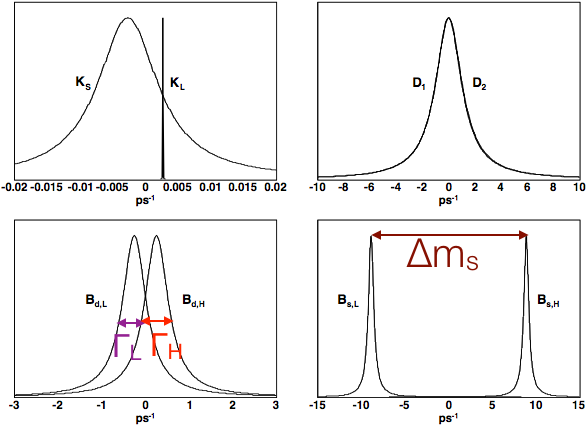
\includegraphics[width=0.7\textwidth]{fig/C_P_CP/MixingMesons}
\caption{Breit Wigner functions describing the lineshapes of the mass eigenstates of mixing neutral mesons systems. The wider the curve, the smaller the lifetime since $\tau = 1/\Gamma$. The peak represents the mass of the particle. The $x$ axis has an offset so that all plots are centred at $0$, so you cannot read off the absolute masses, but you can use it to read off the mass differences and the widths. The units (inverse picoseconds) are a bit unusual, but make it easy to translate this into oscillation frequencies and lifetimes.\label{fig:MixingMesons}}
\end{figure}
Mixing has been observed in Kaons, \Do\ mesons, \Bo\ mesons and \Bso\ mesons. The basic properties (mass and width) of the different meson eigenstates are illustrated in \figref{fig:MixingMesons}. The figure shows the Breit Wigner lineshapes of different mesons. Each lineshape describes the distribution of masses you expect to measure if you observe a large number of particle decays - so there is a mass (energy) uncertainty, represented by the width $\Gamma$ (which is the full width half maximum (FWHM) of these curves). The width is related to the lifetime via $\Gamma = \frac{1}{\tau}$ (or, in SI units, $\Gamma = \frac{\hbar}{c^2\tau}$).  In the plot, the mass is expressed in inverse picoseconds, which might seem a bit peculiar, but given the relationship $\Gamma = \frac{1}{\tau}$, and given that we found earlier that the mixing probability is proportional to $1-\cos\Delta\!m t$, it is quite convenient. The absolute values on the $x$--axis in \figref{fig:MixingMesons} are arbitrary, but the scale is not, so we can read off $\Delta m$ and $\Gamma$.

We observe that for neutral kaons, the most significant difference between the mass/width eigenstates is in the lifetime, which is why we label them by their lifetimes as \Kl\ ("K-long") and \Ks\ ("K-short"). The mass difference is quite slow, so they oscillate very slowly. For both \prt{B} mesons, the widths/lifetimes are very similar, hence we label them as $B_H$ ("B-heavy") and \prt{B_L} ("B-light"). The mass difference between the two \Bso\ states is much bigger than between any of the others, so \Bso\ mesons oscillate very fast. It requires excellent time resolution to measure this. \Do\ mesons, both mass and width are nearly (but not quite) the same, so they oscillate extremely slowly, which is also challenging because you need an incredibly large number of \Do\ mesons to see any hint of an oscillation at all. This is why \Bso\ and \Do\ oscillations were discovered much later than kaon and \Bdo\ oscillations.


\subsection{Mixing and GIM suppression}
\begin{figure}
\begin{tabular}{cc}
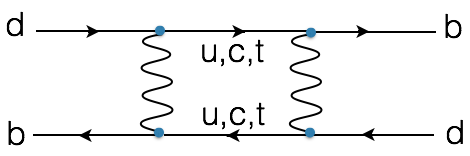
\includegraphics[width=0.4\textwidth]{fig/C_P_CP/BMix1}
&
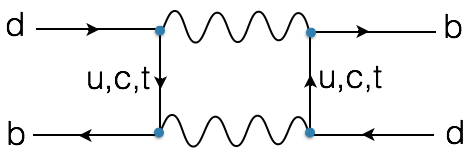
\includegraphics[width=0.4\textwidth]{fig/C_P_CP/BMix2}
\\ a & b
\end{tabular}
\caption{The two box diagrams mediating B mixing.\label{fig:BMixingDiagrams}}
\end{figure}
The Feynman diagrams that allow a \Bo\ to turn into a \Bob\ are given in 
\figref{fig:BMixingDiagrams}.\\
The mixing diagrams such as those for the \Bo\ shown above are clearly flavour changing neutral currents. The same mechanism that suppresses flavour changing neutral currents in the two family model works in principle also with 3 generations of quarks. Instead of $\cos\theta_C$ and $\sin\theta_C$ we now associate the appropriate CKM matrix elements to the vertices, following the rules given in the box on page~\pageref{box:CKMVertices}. For example, we get for the contribution for a loop with two virtual $u$ quark lines: $V_{ud} V_{ub}^* V_{ub}^* V_{ud}$; with two internal $t$ quark lines: $V_{td} V_{tb}^* V_{tb}^* V_{td}$; with a $c$ quark and a $t$ quark: 
$V_{cd} V_{cb}^* V_{td} V_{tb}^*$; etc.
(Note that this is the same for both diagrams shown in \figref{fig:BMixingDiagrams}.) If $u, c, t$ all had identical masses, the sum of the matrix elements would be proportional to the sum of all the relevant products of CKM matrix element. We will now calculate this sum. To make this less messy, we introduce the following notation: $\mathcal{M}_{ij}$ stands for the product of CKM matrix element for the diagram an $i, j$ combination of internal quark lines. We also observe that $\mathcal{M}_{ij} = \mathcal{M}_{ji}$, i.e. for the diagram on the left, you'll find that, in terms of CKM matrix elements it doesn't matter whether the top line is $u$ and the bottom is $\bar{t}$ ($\mathcal{M}_{ut}$) or the top line $t$ and the bottom one $\bar{u}$ ($\mathcal{M}_{tu}$).
\begin{eqnarray}
\lefteqn{\sum\limits_{i=u,c,t}\sum\limits_{j=u,c,t}\mathcal{M}_{ij}}
\nonumber\\
&=& 
\mathcal{M}_{uu} + \mathcal{M}_{cc} + \mathcal{M}_{tt} 
+ 2\left(\mathcal{M}_{uc} + \mathcal{M}_{ut} + \mathcal{M}_{ct}\right)
\nonumber\\
&=& V_{ud}^2 V_{ub}^{*2} 
+ 
V_{cd}^2 V_{cb}^{*2}
+
V_{td}^2 V_{tb}^{*2}
+
2 \left(
V_{ud} V_{ub}^{*}V_{cd} V_{cb}^{*}
+ V_{ud} V_{ub}^{*}V_{td} V_{tb}^{*}
+V_{cd} V_{cb}^{*}V_{td} V_{tb}^{*}
\right)
\nonumber\\ &=&
\left(V_{ud} V_{ub}^{*} 
+ 
V_{cd} V_{cb}^{*}
+
V_{td} V_{tb}^{*}\right)^2
\nonumber\\ &=& 0
\end{eqnarray}
where in the last step, we used the unitarity relations given in Equations~\ref{eq:CKMUnitarity}. 

\exercise{Draw the equivalent Feynman diagrams for Kaon mixing and D meson mixing, and repeat the exercise, i.e. show that if all quark masses were the same, the sum of the mixing diagrams over all internal quark lines would be zero.}

So if all up-type quark masses were the same, the GIM cancellation would work perfectly even in three (or more) generations, as long as the mixing matrix is unitary. But of course the quark masses are not equal.
Especially, the top quark mass is huge (\un{175}{GeV} compared to $0$ ish for the $u$ and few GeV for the $c$ quark). As a consequence, and combined with the large value of $V_{tb}$, the top contribution completely dominates the \Bo--\Bob\ mixing diagram. 
A rough numerical estimate for the different contributions can be obtained by multiplying the approximate magnitude of the CKM elements with the mass of the internal quark.
\begin{itemize}
 \item For the $d \to t \to b$ transition this is is $\sim \lambda^3 m_t$.
 \item For the $d \to c \to b$ transition this is $\sim \lambda^4 m_c$
 \item For the $d \to u \to b$ transition this is $\sim \lambda^3 m_u$
\end{itemize}
 If you now take into account that the top is $\sim 100\times$ as
 heavy as the charm, and $100,000$ times as heavy as the $u$ quark,
 it is clear that the top contribution completely dominates and we can neglect the contributions of the other
 quarks. The same is true for \Bso\ mixing. This will simplify the calculations we'll do with these diagrams, later. For the kaon mixing diagram, the picture is a bit more murky, because $V_{ts}$ is quite small. And for charm mixing, we need to look at GIM cancellation with internal $d, s, b$ quarks, which works better (the range of masses is much more restricted), plus the $b$ quark contributions are suppressed because they involve only small CKM matrix elements. 
The consequence of all of this is that \Bo\ and \Bso\ oscillations are quite fast (especially \Bso
 - they were so fast that it took until 2006 for them to be discovered), while Kaon oscillations are quite slow, and \Do\ oscillations are extremely slow (so slow it took until 2007 for them to be discovered). In fact the measurement of the \Bdo\ oscillation frequency was used to estimate the top mass long before the top had been produced directly.

And why did 2-generation GIM cancellation ever work? Because of the coincidence that the CKM matrix nearly has a $2 + 1$ block structure:
\[
V_{CKM} \sim \parbox{0.2\textwidth}{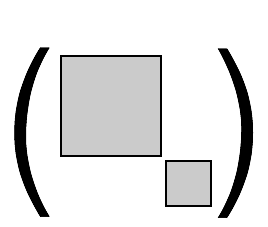
\includegraphics[width=0.2\textwidth]{fig/CKM_block}}
\]
which means that both the $2\times 2$ block and the $1\times 1$ block are approximately separately unitary, to a good enough approximation at least that GIM worked fairly well when it was conceived. But it's important to remember that it's those small off-diagonal elements, which destroy this simple picture, that couple the 3rd generation of quarks to the other two, and are responsible for CP violation.

\section{Manifestations of \cpv, \cpv\ measurements}
\label{sec:CPVinB}
 In the SM, the CKM matrix is the only source of \cp\ violation. Therefore, all \cp\ violation measurements have to measure the phases of the CKM
 matrix. We remember from basic Quantum Mechanics that absolute phases
 cannot be measured, so what we need is phase differences. Phase
 differences show up in interference experiments (remember the double
 slit experiment - all what follows will in essence be that).

 \textbf{All CP violation measurements are interference experiments}
 where we have more than one path from an initial state to a final state, and the
 phase difference between the two (or more) paths shows up in the measured decay
 rates.
 
 \fbox{\parbox{0.9\textwidth}{\paragraph{Which CKM phases} If you want to figure out which CKM phases (e.g $\beta, \gamma$ or a combination like $2\beta -\gamma$) a certain decay is sensitive to, find out which decay diagrams could interfere and find out their CKM phases. If a \cpv\ parameter can be measured in this decay, it will be the phase difference between those two diagrams - even if you don't know at all how the measurement is done in practice}}
 
 In this section we will concentrate on \cpv\ in B hadrons. This is where \cpv\ effects are largest, and this is also where they can be connected best to specific CKM parameters.
 
\subsection{Types of \cp\ violation}

\subsubsection{CP violation in the mixing ("indirect CP violation")}
This is when the mass/width eigenstates do not match the CP eigenstates.
This is the dominant type of CP violation in the kaon system. This is expressed by the parameter $\epsilon$ in 
\begin{eqnarray}
\ket{\Kl} &=& \frac{1}{\sqrt{1 + \epsilon^2}} \left(
             \ket{K_{\mathsf{odd}}} + \epsilon \ket{K_{\mathrm{even}}} \right)
             \nonumber\\
\ket{\Ks} &=& \frac{1}{\sqrt{1 + \epsilon^2}} \left(
             \ket{K_{\mathsf{even}}} - \epsilon \ket{K_{\mathrm{odd}}} \right)
\end{eqnarray}
where $\epsilon$ is small, about $2.2\E{-3}$.
This is often also called "indirect \cpv". This type of \cpv\ is negligible in \Bdo\ and \Bso\ meson decays.

\paragraph{What interferes with what?}
$K^0 \to K^0$ with $K^0 \to \bar{K}^0 \to K^0$

(Sidenote: There is also direct \cpv\ in the kaon system, it's even smaller than indirect \cpv\ and it's measured by $\epsilon'$. This was historically very important, but we will not look into this parameter in this course, as there are much "cleaner" (easier to interpret in terms of CKM phases) direct \cp\ violation measurements in B meson decays.)

\paragraph{Indirect \cpv\ in the $B$ system}


In the $B$ system (($B^0$, or $B_s$) indirect \cpv\ is expected to be very small in the SM due to the CKM factors involved in the mixing. However sources beyond the SM can induce large indirect \cpv\ effects.
The typical way that experimentalists try to measure \cpv\ the $B$-system is through the ``flavour-specific" decays of $B^0\to D^-\mu^+\nu_{\mu}$ or  $B_s \to D_{s}^{-}\mu\nu_{\mu}$. These types of decays are called flavour specific because of the fact that for instance, the $B^0$ cannot decay to $D^+\mu^-\bar{\nu}_{\mu}$ but the $\bar{B}^0$ can (due to conservation of electric charge). This means that one can identify the whether the $B$-meson was a $B^0$ or a $\bar{B}^0$ when it decayed, simply by looking at the decay products. Another way of saying this, is that the amplitude 
\begin{equation}
\bra{B^{0}}\hat{H}_{W}\ket{D^+\mu^-\bar{\nu}_{\mu}} = \bra{\bar{B}^{0}}\hat{H}_{W}\ket{D^-\mu^+\nu_{\mu}} = 0
\end{equation}
where $\hat{H}_{W}$ is the weak Hamiltonian that mediates the decay.

As indirect \cpv\ would imply that the rate of $B\to\bar{B}$ is different compared to that of $\bar{B}\to B$, it is also important to know the flavour of the $B$ when it was produced. This is done by using a range of techniques (depending on the experiment). It is called flavour-tagging and the details of this method are beyond the scope of this course. 

Armed with the flavour of the $B$ at production and decay, experimentalists can measure the asymmetry $a_{sl}$ (``$sl$" for semileptonic owing to the final state of the $B$) given by
\begin{equation}
a_{sl}=\frac{\Gamma(\bar{B}^{0}\to B^0\to  D^-\mu^+\nu_{\mu}) - \Gamma(B^{0}\to \bar{B}^0\to  D^+\mu^-\bar{\nu}_{\mu})}{\Gamma(\bar{B}^{0}\to B^0\to  D^-\mu^+\nu_{\mu}) + \Gamma(B^{0}\to \bar{B}^0\to  D^+\mu^-\bar{\nu}_{\mu})} = \frac{1-|q/p|^4}{1+|q/p|^4}
\end{equation}
In the absence of indirect \cpv\, $a_{sl}=0$ and therefore $|q/p|=1$ as we discussed in Sec~\ref{sec:bosc}.


\subsubsection{CP violation in the decay ("direct \cpv")}
This is when the decay rates for some initial state $i$ to a final state $f$ are not the same as for the \cp--conjugate decay. For example
\[
\Gamma(\Bm \to (\Kp\pim)_D K^-) \neq \Gamma(\Bp \to (\Km\pip)_D K^+) 
\]
is a case of large direct \cpv\ discussed in detail further below.

In general, direct \cpv\ occours when two or more decay amplitude interfere. $A_i e^{\phi_i + \delta_i}$ with magnitude $A_i$,  CP-violating phases $\phi_i$ and CP-conserving phases (due to the strong interaction) $\delta_i$, rates for the process $B\to f$ described by the sum of these amplitudes are given by:
\begin{equation}
\Gamma(B \to f) \propto \left| A_1 e^{i\left(\phi_1 + \delta_1\right)} + 
|A_2 e^{i\left(\phi_2 + \delta_2\right)} \right|^2
= A_1^2 + A_2^2 + 2 A_1 A_2 
\cos(\Delta \delta + \Delta \phi)
\end{equation}
where $\Delta\delta = \delta_1 - \delta_2$ and $\Delta \phi = \phi_1 - \phi_2$. Under CP we find
\begin{equation}
\Gamma(\overline{B} \to \overline{f}) \propto \left| A_1 e^{i\left(-\phi_1 + \delta_1\right)} + 
|A_2 e^{i\left(-\phi_2 + \delta_2\right)} \right|^2
= A_1^2 + A_2^2 + 2 A_1 A_2 
\cos(\Delta \delta - \Delta \phi)
\end{equation}

A notable feature is that direct \cpv\ requires not only a phase difference in CKM phases, but also in the strong interaction.

\paragraph{What interferes with what?} 
$A_1 e^{\phi_1 + \delta_1}$ with $A_2 e^{\phi_2 + \delta_2}$, both amplitudes with the same initial and final state. For example:
$\Bm \to \Do \Km, \Do \to \Kp\pim$ with $\Bm \to \Dob \Km, \Dob \to \Kp\pim$


\subsubsection{CP violation in the interference between mixing and decay}
 The \emph{classic} \cp\ violation experiment in B physics makes use
 of the ``interference between decay and mixing''. At the basis of the
 measurement is B mixing, which allows a \Bdo\
 meson to change into a \Bdob\ meson. This works for other neutral
 meson systems, too, like \Bso\ mesons or neutral Kaons.

 Then need a decay that is accessible to both, \Bdo\ and \Bdob. A
 \cp\ eigenstate is a good pick. Let's call it $f_{CP}$. Now, if we
 have two decay paths to the same final state:
\begin{enumerate}
 \item \prt{\Bdo \to f_{CP}}
 \item \prt{\Bdo \to \Bdob \to f_{CP}}
\end{enumerate}
 The interference effects between the two path let us measure \cp\ violating phases.
\paragraph{What interferes with what?}
\prt{\Bdo \to f} with \prt{\Bdo \to \Bdob \to f}

\subsubsection{The \prt{\Bo \to \Bob} box diagrams}
 What phase do we measure with this? It is the phase difference
 between the two decay paths. So we need to establish what phase is
 picked up in the \prt{\Bdo \to \Bdob} transition, and add to that the
 phase difference between \prt{\Bdo \to f_{CP}} and \prt{\Bdob \to
 f_{CP}}. For the latter we'll have to pick a specific final state for
 $f_{CP}$. But we'll start with the \prt{\Bdo \to \Bdob} transition,
 that is the same in all measurements of this kind.

 For this we write down the Feynman diagram for the \prt{\Bdo \to
 \Bdob} transition:
\begin{equation}
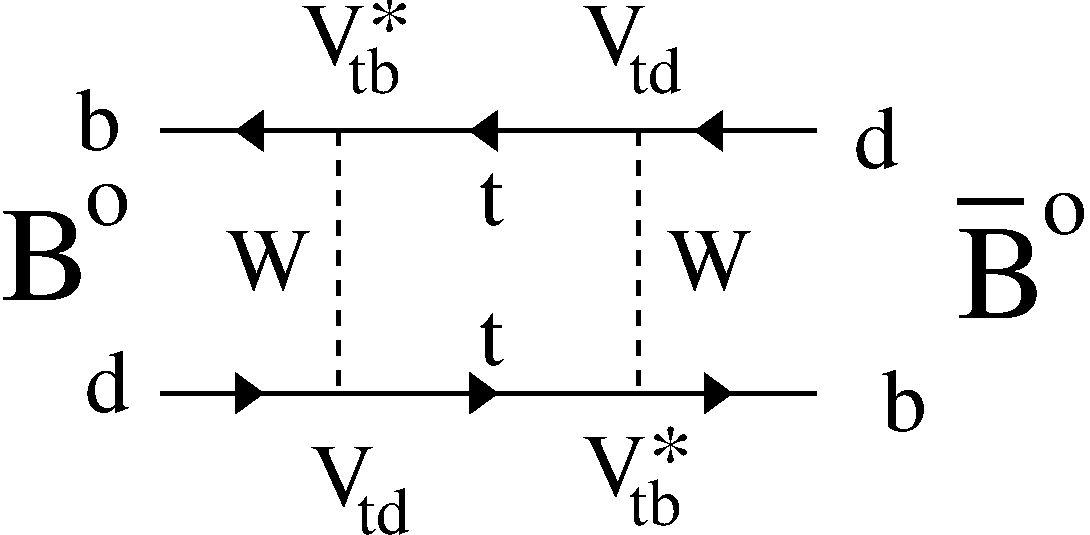
\includegraphics[width=0.5\textwidth]{fig/C_P_CP/feyn_mix_bw.pdf}
\end{equation}
 This is the famous \textbf{Box Diagram} for B mixing.

 Let's go step by step through this diagram:
\begin{itemize}
 \item Time flows from left to right.
 \item Arrows pointing from right to left indicated
 anti-particles. This is an awkward notation - it means that the b
 quark line on top is in fact a $\bar{b}$. It stems from the fact
 that, because of \cpt\ invariance, \cp\ should be the same as \ts. So
 instead of writing down $\bar{b}$ we ``just'' invert the arrow of time.
 Note that some authors will draw all arrows going from left to write
 and a bar over the $b$. That's OK. And many will do both, write
 $\bar{b}$ and the arrows from right to left - that is technically
 wrong, but is intended to mean the same thing, and if you want, you can also use that system, I'm not going to be too fussy.
 \item Another piece of awkward notation: A \Bdo\ meson is made of
 $\bar{b}, d$ and a \Bdob\ meson of $b, \bar{d}$.
 \item And finally, this is a so-called loop diagram. The loop is the
 box. Inside loops, the usual constraints that the decaying particle
 must be heavier than the sum of the products don't apply. That's why
 the $d\to t$ transition is allowed - because the $t$ is inside a
 loop.
\end{itemize}

We recognise the above diagram as
one that describes a \prt{\Bdo \to \Bob} transition. To establish the
phase of this diagram
\begin{itemize}
 \item At each vertex, write down the appropriate CKM matrix
 element
 \item Multiply them together, or equivalently, if it's only the phase
 you're after, add up the phases.
 \item For the above diagram, the elements and their phases are (we
 only go to \order{\lambda^3} in the Wolfenstein parameterisation):
 \begin{itemize}
 \item $V_{td} \propto e^{-i\beta}$
 \item $V_{tb}^* \propto e^{-i 0}$
 \item $V_{td} \propto e^{-i\beta}$ (again)
 \item $V_{tb}^* \propto e^{-i 0}$ (again)
 \end{itemize}
 So the total phase of this diagram is $-2\beta$.
\end{itemize}

 There is another diagram, the equally famous other \textbf{Box
 Diagram} for B mixing that also contributes to B mixing:
\begin{equation}
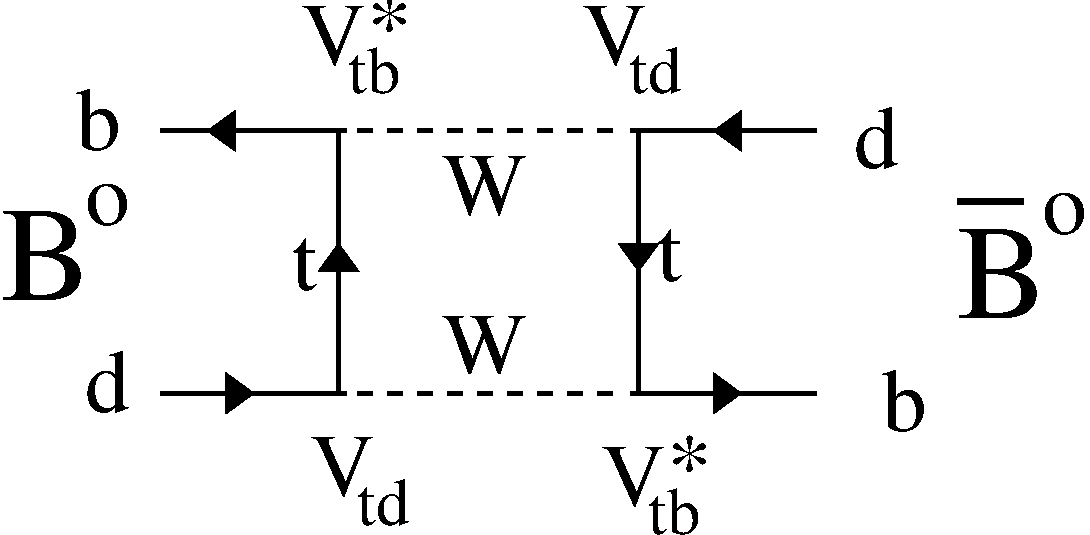
\includegraphics[width=0.5\textwidth]{fig/C_P_CP/feyn_mix2_bw.pdf}
\end{equation}
 If you repeat the exercise above, you'll find that it has exactly
 the same phase, so adding the two diagrams together still has a phase
 of $-2\beta$.

As we discussed above, the top contribution completely dominates (and two tops completely dominate over one) so that we can neglect diagrams like these:
\begin{equation}
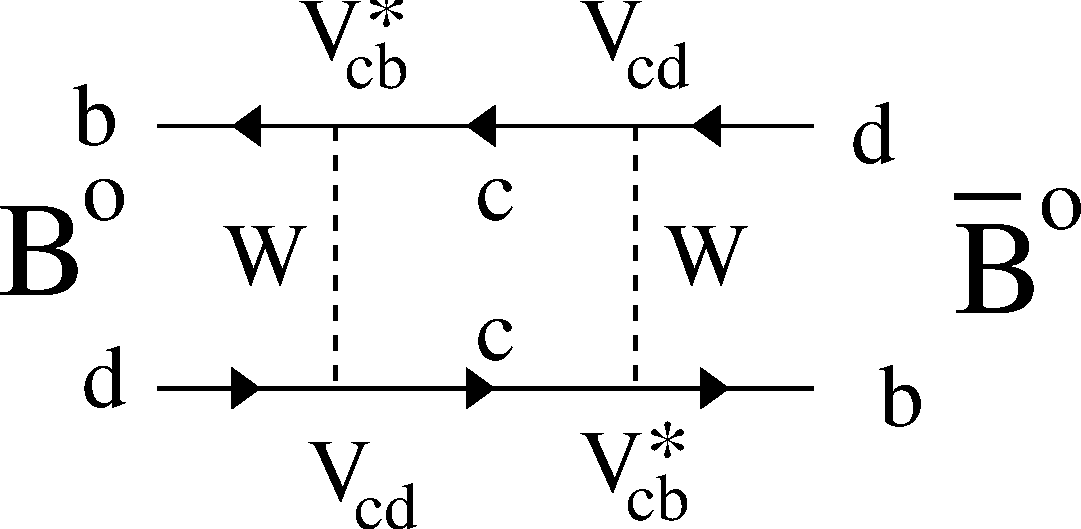
\includegraphics[width=0.3\textwidth]{fig/C_P_CP/feyn_mix_c.pdf}
\;\;
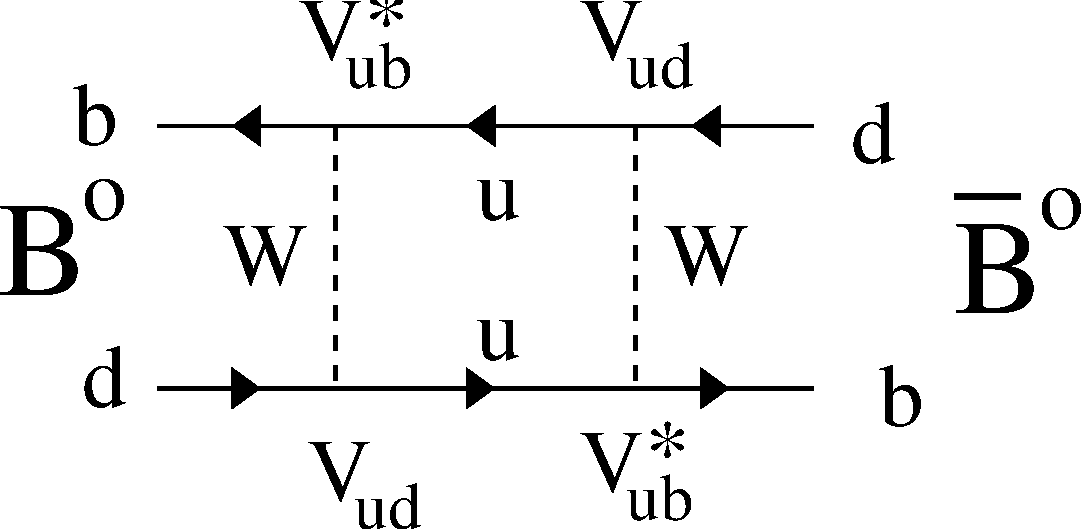
\includegraphics[width=0.3\textwidth]{fig/C_P_CP/feyn_mix_u.pdf}
\;\;
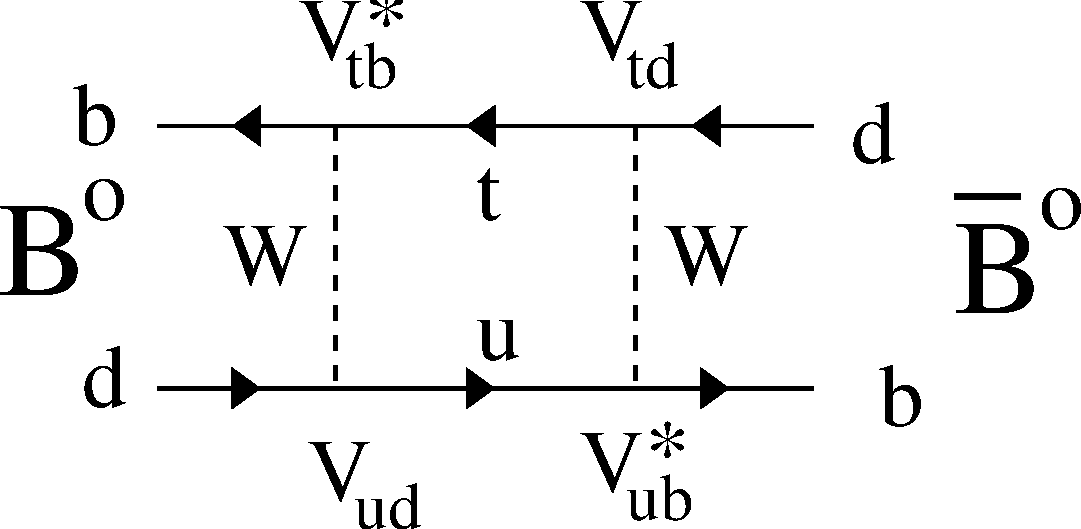
\includegraphics[width=0.3\textwidth]{fig/C_P_CP/feyn_mix_tu.pdf}
\end{equation}

\subsubsection{For example \prt{f_{CP} = K_s J/\psi}}

 The J/psi is a $c\bar{c}$ bound state - this is the particle that was
 actually seen when the charm quark was discovered. It has $J^{PC} =
 1^{--}$, it is a \cp\ even eigenstate. The $K_s$... well, because of
 \cp\ violation in the Kaon system, the $K_s$ is not a \cp\ eigenstate
 at all. But because \cp\ violation in the Kaon system is so much
 smaller than in the B system, for the purpose of this example, we
 can neglect this effect for now and assume that \Ks\ is \cp\ even. In real
 measurements, a correction for the small \cp\ violation in the Kaon
 system is applied, but it is really very small.

 So we have a CP-even eigenstate. But what does it contribute to the
 phase difference between
\begin{enumerate}
 \item \prt{\Bdo \to J/\psi K_s}
 \item \prt{\Bdo \to \Bdob \to J/\psi K_s}?
\end{enumerate}

 The tree-level (= no loops) diagram that contributes to this decay is:
\begin{equation}
 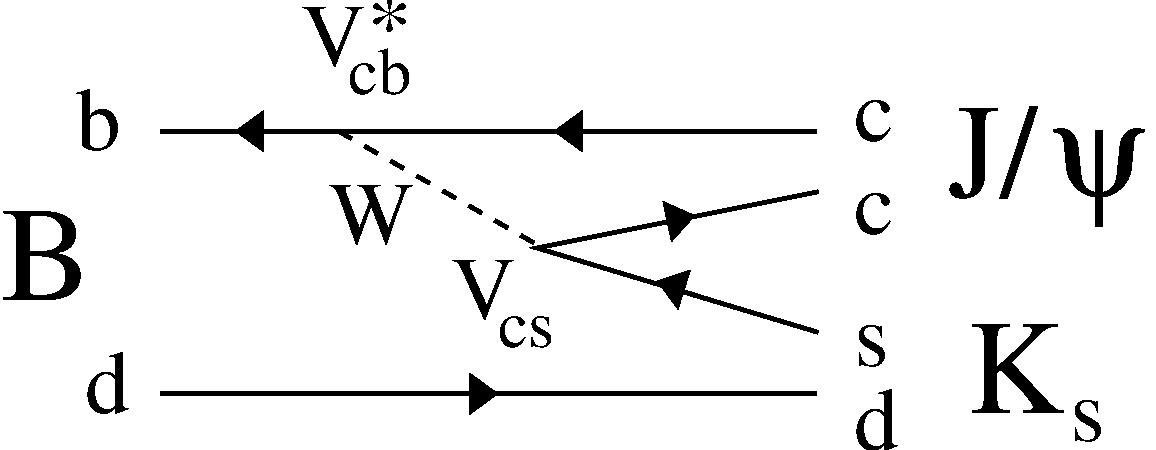
\includegraphics[width=0.5\textwidth]{fig/C_P_CP/feyn_btojpsiK_bw.pdf}
\end{equation}
 A few remarks about this one: The decay we drew is actually one with
 a $K^0$ in the final state - this has (neglecting \cp\ violation in
 the Kaon system) a 50\%- 50\% chance of decaying as a $K_s$ or a
 $K_L$. The way we know that it was a $K_s$ is that it decays within
 the detector volume. A $K_L$ would live too long to do that, and just
 escape.

 This diagram is proportional to $V^*_{cb} V_{cs}$, so (up to
 \order{\lambda^3}), it has phase $0$.
  
 The \cp-conjugate diagram, \prt{\Bob \to J/\psi K_s}, is 
\begin{equation}
 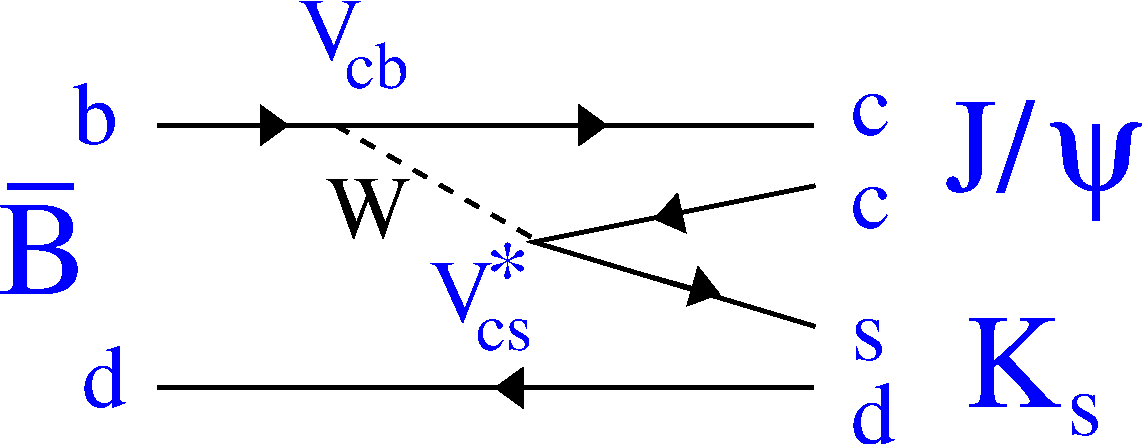
\includegraphics[width=0.5\textwidth]{fig/C_P_CP/feyn_bbbartojpsik.pdf}
\end{equation}
 This has also the phase $0$. We could have known that w/o writing
 down the diagram, of course - the weak phase of the \cp\ conjugate
 process is just the negative of the original process.

There is another contribution to this decay, the so-called penguin
diagram. This looks like so:
\begin{equation}
 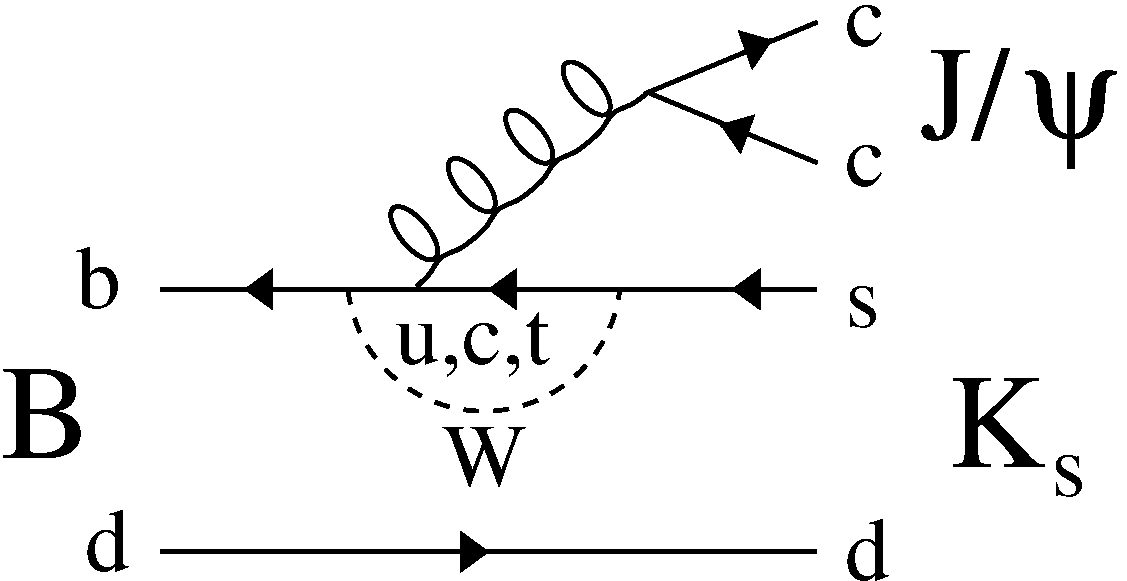
\includegraphics[width=0.5\textwidth]{fig/C_P_CP/feyn_btojpsiK_penguin_bw.pdf}
\end{equation}
 This is a loop diagram, and again it is the top quark that
 dominates the loop, and there is no phase from the corresponding matrix elements $V_{tb}^* V_{ts}$. This is one of the the reasons why $J/\psi \phi$ is referred to as the "golden mode" for measuring $\beta$: Both penguin and tree contribution have the same, zero phase. (The other reason is that the $J/\psi$ can be experimentally very cleanly reconstructed in the decay mode $J/\psi \to \mu^+ \mu^-$).)
 
\subsubsection{The strong phase}
 We neglected up to now that each decay diagram also involves the
 strong interaction, which is responsible for binding the quarks
 together into the observable mesons. But since the strong interaction
 is \cp\ symmetric, there won't be a strong phase difference between
 the two \cp\ conjugate decays \prt{\Bo \to J/\psi K_s} and \prt{\Bob
 \to J/\psi K_s}. So the overall phase difference between the two is
 zero.
\subsubsection{Putting it all together}
 So, the overall phase difference between the decays
\begin{enumerate}
 \item \prt{\Bdo \to J/\psi K_s}
 \item \prt{\Bdo \to \Bdob \to J/\psi K_s}
\end{enumerate}
 is $-2\beta$ from the mixing diagram, and $0$ from the decay
 diagrams.\footnote{We did not look at any phases due to the strong interaction - these can affect the decay but they do not matter here. The strong interaction is \cp\ conserving, so any strong phase that would be the same in \prt{\Bo \to J/\psi K_S} and the \cp-conjugate process \prt{\Bob \to J/\psi K_S} (remember that \prt{J/\psi K_S} is a \cp\ eigenstate). So here, any strong phases cancel in the phase difference.}
 This can be visualised like this
\\
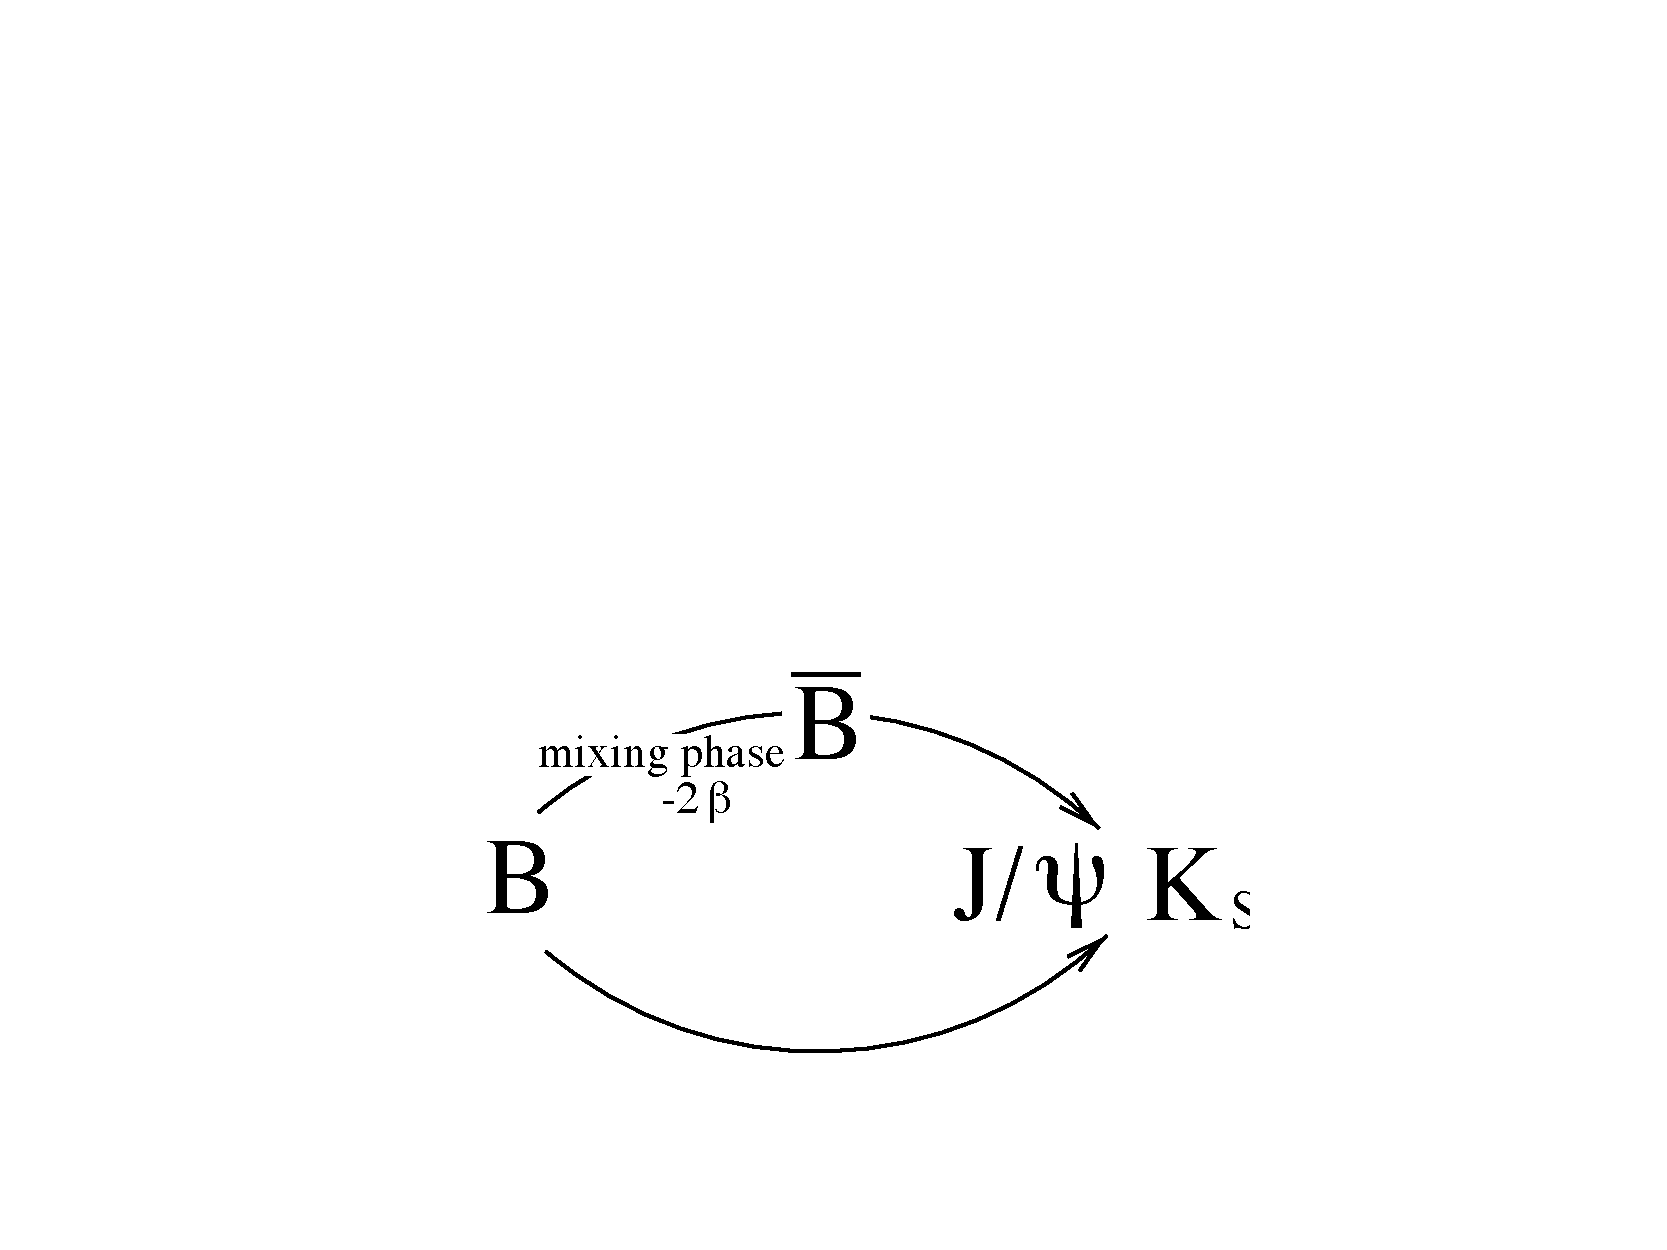
\includegraphics[width=0.5\textwidth]{fig/C_P_CP/B2JpsiKs_beta}
\\
 The fact that all contribution to the decay mode (both,
 tree and penguin) enter with the same phase, makes it \textbf{The
 golden mode} for measuring the CKM phase $\beta$.

 So we established now that the measurable quantity in \prt{\Bdo \to
 J/\psi K_S} decay is $-2\beta$. But how is it measured? It is measured in time dependent decay rate asymmetries:
\begin{equation}
\label{eq:timedepasy}
A\!\left(t\right) =
\frac{   \Gamma\left(\Bo \to f \right)(t)
        -\Gamma\left(\Bob \to f \right)(t)
    }{
         \Gamma\left(\Bo \to f \right)(t)
        +\Gamma\left(\Bob \to f \right)(t)
    }
\end{equation}
 Such ratios are experimentally favourable because acceptance effects
 etc cancel in the ratio.
 In decays to \cp\ eigenstates, $A(t)$ is given by
\begin{equation}
 A(t) = \mp \sin(\phi) \; \sin(\Delta\!m\, t)
\end{equation}
 where $\phi$ is the phase difference between the two decay paths, the one via mixing and the one without. For \prt{\Bdo \to
 J/\psi K_S}, $\phi = -2\beta$.
 
% \begin{figure}
% \includegraphics[width=0.5\textwidth]{fig/BELLE_B2JpsiKsAsy}
% \caption{Time-dependent decay rate asymmetry (\eqnref{eq:timedepasy}) in \prt{B^0 \to J/\psi K_S} (and related decays) as measured by the BELLE experiment in 2012. \href{https://inspirehep.net/record/1085529?ln=en}{Phys.Rev.Lett. 108 (2012) 171802}.\label{fig:tddra}}
% \end{figure}
 \begin{figure}
 \centering
 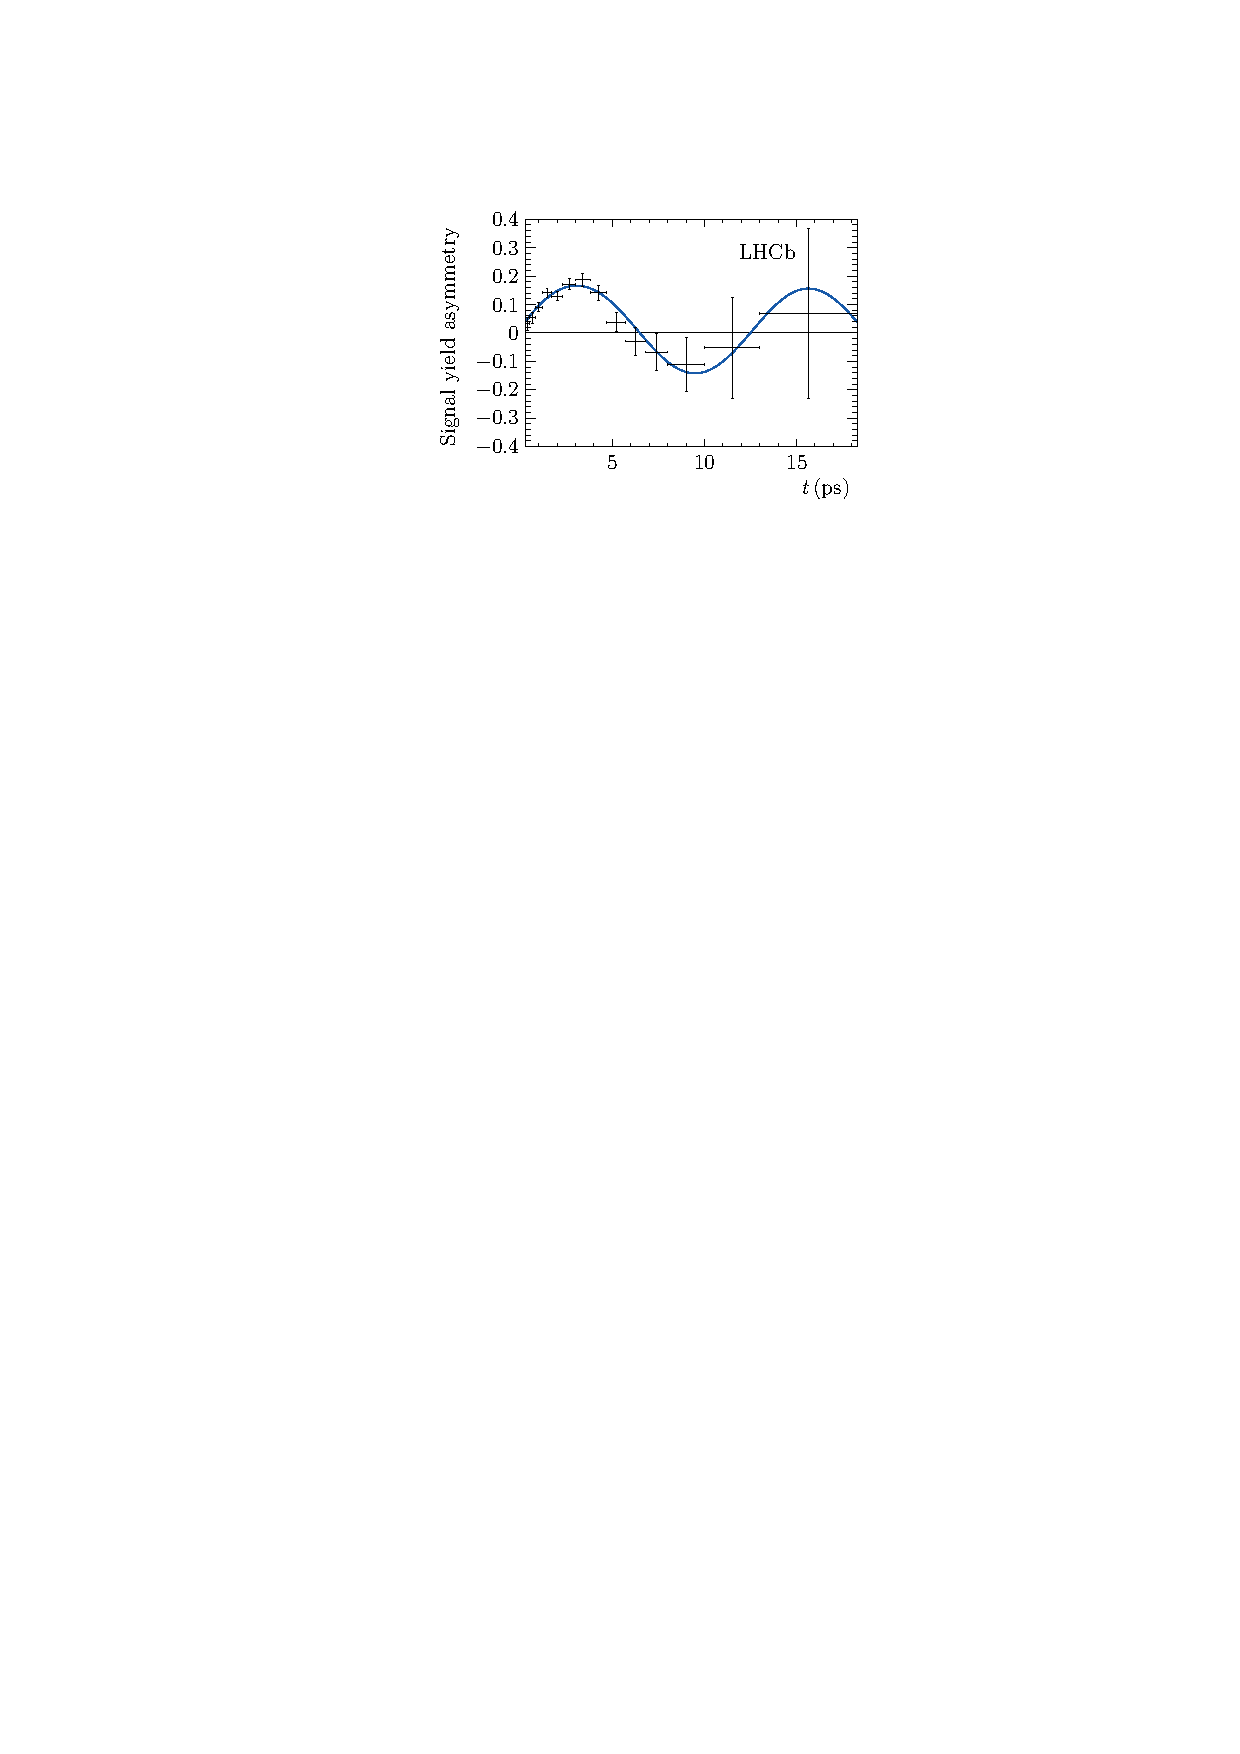
\includegraphics[width=0.6\textwidth]{fig/LHCb_B2JpsiKsAsy}
 \caption{Time-dependent decay rate asymmetry (\eqnref{eq:timedepasy}) in \prt{B^0 \to J/\psi K_S} (and related decays) as measured by the LHCb experiment in 2015 (\href{http://inspirehep.net/record/1355375/}{Phys.Rev.Lett. 115 (2015) no.3, 031601}). 
 The first (and still most precise) measurements of $\sin2\beta$ quantity are from BaBar
 and BELLE (both now stopped data taking, for their final results, see \href{https://inspirehep.net/record/812984?ln=en}{Phys.Rev. D79 (2009) 072009} \href{https://inspirehep.net/record/1085529?ln=en}{Phys.Rev.Lett. 108 (2012) 171802}). 
 The current world-average for $\sin(2\beta)$ from this type of measurement is $0.691 \pm 0.017$.
 The reason the amplitude in the plot is much smaller than $0.961$ is "mistag", mis-identification of \prt{B^0} and \prt{\overline{B}^0} at $t=0$. By knowing the probability for this to happen precisely, this can be corrected.
% corresponding to $\beta = 21.9^{\circ} \pm 0.7^{\circ}$ or $\beta = 68.1^{\circ}\pm 0.7^{\circ}$ (the other two values for $\beta$ compatible with $\sin(2\beta)=0.691\pm 0.017$ are excluded by  other measurements showing $\cos2\beta > 1$).
 For more results and averages, see \href{http://www.slac.stanford.edu/xorg/hfag/triangle/summer2016/index.shtml\#sin2b}{HFAG}.\label{fig:tddra}}
 \end{figure}
 \subsubsection{Summary of \cp\ violation in the interference between
 mixing and decay}
\label{sec:BCPSummary}

\begin{itemize}
 \item Mixing itself is not CP violating.
 \item By choosing the right decay mode, you can pick what you want to
 look at, \Bh, \Bl or \Bo, \Bob. Decays to flavour eigenstates see the
 \Bo, \Bob\ aspect and therefore the oscillation.
 \item Decays to \cp\ eigenstates would see \Bh\ and \Bl, if there were
 no CP violation - w/o CP violation no oscillation would be seen in
 such decays. The size of the oscillation that \emph{is} seen in decays to CP
 eigenstates measures \cp\ violation.
 \item The oscillation is best measured in ``time dependent decay rate
 asymmetries''. That is the number of \prt{\Bdo \to f} decay minus
 \prt{\Bdob \to f} decays divided by their sum, as a function of time,
 where \Bdo\ and \Bdob\ refers to the flavour at time
 $t=0$. Mathematically:
\begin{equation}
\label{eq:defasy}
A\!\left(t\right) =
\frac{   \Gamma\left(\Bo \to f \right)(t)
        -\Gamma\left(\Bob \to f \right)(t)
    }{
         \Gamma\left(\Bo \to f \right)(t)
        +\Gamma\left(\Bob \to f \right)(t)
    }
\end{equation}
 Such ratios are experimentally favourable because acceptance effects
 etc cancel in the ratio.
 \item In decays to \cp\ eigenstates, $A(t)$ is given by
\begin{equation}
 A(t) = \mp \sin(\phi) \; \sin(\Delta\!m\, t)
\end{equation}
 Where $\phi$ is the phase difference between the two interfering
 decay paths that we calculated above for the case of \prt{f=J/\psi
 K_s} where it is $-2\beta$.  The sign in front of $\sin(\phi)$
 depends on whether it is a CP-even or odd final state. For \cp\ even
 final states it's $-$, for \cp\ odd states it is $+$.
\item All of the above works for \Bdo\ as well as for \Bso\ (if you take
  into account the non-zero lifetime difference in \Bso\ system between \Bsl\
  and \Bsh, a few extra terms come into play - while these do
  matter for a precision measurement, we can ignore them for now).
\end{itemize}

To distill this even further:
\begin{itemize}
 \item \cp\ violation can be measured by measuring the
 \textbf{amplitudes of time dependent decay rate asymmetries}.
 \item For decays to \cp\ eigenstates \textbf{the amplitude of the
  asymmetry is the sine of the phase-difference between the
  interfering decay paths}.
\end{itemize}

 \subsection{Direct \cp\ violation (example question \& answers)}
\begin{enumerate}[a)]
\item Consider the decays \prt{B^- \to D^0 K^-} and \prt{B^- \to \overline{D}^0 K^-}. 
 \begin{itemize}
 \item Use the formula sheet to find out the quark content of the mesons involved.
 \answerbox{
 $\prt{B^-} = (b, \overline{u})$, \\
 $\prt{D^0} = (c, \overline{u})$ (and hence $\prt{\overline{D^0}} = (\overline{c}, u)$,\\
 $\prt{K^-} = (s, \overline{u})$.
 }
 \item Draw the tree-level Feynman diagrams that describe these decays. There are two topologies, they look like this:\\
 \begin{tabular}{cc}
 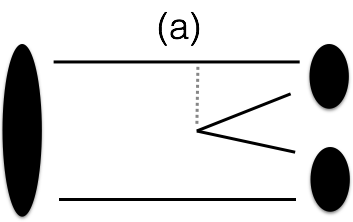
\includegraphics[width=0.3\textwidth]{problemsheets/ps2figs/CSup} &
 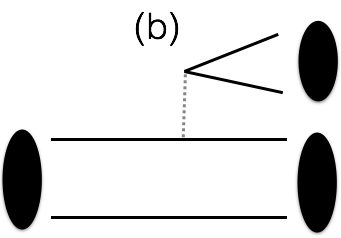
\includegraphics[width=0.3\textwidth]{problemsheets/ps2figs/CFav}
 \end{tabular}\\
 where the black blobs indicate that two quarks form a meson.
 \answerbox{The diagrams look like this:\\
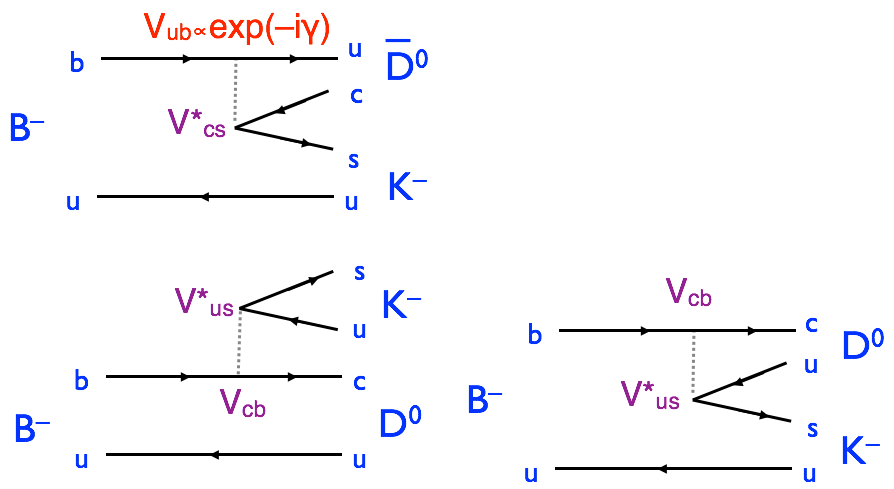
\includegraphics[width=0.7\textwidth]{problemsheets/ps2figs/B2DKDiagrams.png}
}
 \item One of the topologies for the \prt{B^-} decay diagrams given above is "colour-suppressed". This means that the requirement that mesons are colourless objects restricts the colours that the quarks that result from this decay can have (while for the other diagram there is no such restriction). Which topology is colour suppressed? Explain, why.
 \answerbox{ (Remember, quarks can be red, green, blue, anti-quarks can
  be anti-red, anti-green, anti-blue; colourless objects can be made
  by combining three quarks: red + green + blue = white; or three
  anti-quarks: anti-red, plus anti-green plus anti-blue is also white;
  or by combining quark-antiquark pairs like red + anti-red, or green
  + anti-green, or blue + anti-blue.)
  \vspace{2ex}\\
  Topology (a) is colour suppressed. This is because in this diagram:
  \\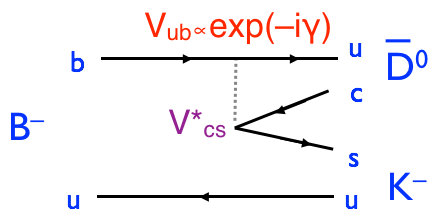
\includegraphics[width=0.5\textwidth]{problemsheets/ps2figs/B2DK_supp}\\
  the \prt{B^-} is colour neutral, so it is a colour - anti-colour
  pair (say red and anti-red). The $\overline{c}$ and $s$ quark must
  then have the same anti-colour/colour as the $\overline{b}$ and $u$
  quark we started off with, in order to produce colour-less mesons
  (in our example anti-red, red). The \prt{B^-} is colourless, so if,
  for example, the $b$ is red, than the $\overline{u}$ must be anti-red }
 \item One of the two decays can proceed via both topologies (colour favoured and colour suppressed), the other only by one of them. To simplify the rest of the question a bit: for the decay where both topologies apply, only consider the colour favoured diagram and ignore the suppressed.
 \answerbox{... so this means that you should only consider these two diagrams:
 \\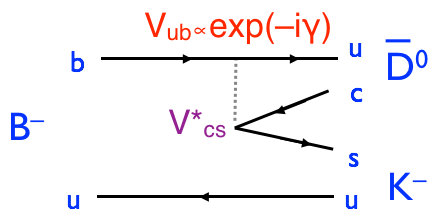
\includegraphics[width=0.4\textwidth]{problemsheets/ps2figs/B2DK_supp}, 
 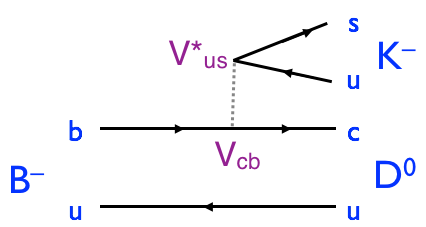
\includegraphics[width=0.4\textwidth]{problemsheets/ps2figs/B2DK_fav}.
 }
 \item Estimate the complex value of the ratio of the two diagrams
  \[
    r_B e^{i\phi} = \frac{A(\prt{B^- \to \Dob K^-})}{\prt{A(B^- \to \Do K^-})}
 \]
 expressed as a magnitude $r_B$ and phase $\phi$. You obtain this value
 by multiplying together the vertex factors and multiplying the colour-suppressed diagram by $1/\sqrt{3}$ to take into account the colour suppression. 
 \end{itemize}
 \answerbox{
    The value of the \prt{\Bm \to \Dob \Km} diagram (i.e. the product of the relevant vertex factors) is $g_W V_{ub} \cdot g_W V^*_{cs}$. For \prt{\Bm \to \Dob \Km} it is $g_W V_{cb} \cdot g_W V_{us}^*$. The colour suppression introduces an additional factor of $1/\sqrt{3}$ to the \prt{\Bm \to \Dob \Km} diagram. So the ratio is:
    \[
    r_B e^{i\phi}  = \frac{A(\prt{B^- \to \Dob K^-})}{\prt{A(B^- \to \Do K^-})} = 
    \frac{V_{ub} \cdot V^*_{cs}}{\sqrt{3} \; V_{cb} \cdot V_{us}^*}
    \]
    From the formula sheet: 
    \begin{itemize}
     \item $V_{ub}   = 0.0037 \cdot e^{-i\gamma}$
     \item $V_{cs}^* = 0.97$
     \item $V_{cb}   = 0.041$
     \item $V_{us}^* = 0.23$
    \end{itemize}
    With this I get: $r_B e^{i\phi} = 0.22 e^{-i\gamma} = 0.22 e^{-i (68^{\circ})}$
 }
%%
\item Now consider the decay chains
\prt{B^- \to D^0 K^-, \Do \to K^+ K^-} and \prt{B^- \to \overline{D}^0 K^-, \Dob \to K^+ K^-}.
 \begin{itemize}
 \item Note that these two decay paths will interfere with each other - the situation is analogous to the double slit experiment:
 \\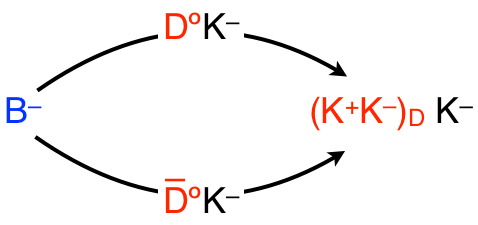
\includegraphics[width=0.5\textwidth]{problemsheets/ps2figs/B2DK_D2KK_interference}
 \item A bit of notation: To refer to the full decay that includes the interference between these decay paths, we write
 \prt{B^- \to (K^+ K^-)_D K^-}.
 Here, the notation \prt{(K^+K^-)_D} simply indicates that the \prt{K^+} and \prt{K^-} result from the decay of the \Do\ or \Dob. 
 \item Interference leads to sensitivity to phases - specifically, to sensitivity to the phase difference between the two decay paths. Your Feynman diagrams should indicate a phase difference of $\phi = -\gamma$ due to the weak interaction. This, however, neglects the effects of the strong interaction. This is difficult to calculate but it also leads to a phase difference, which we call $\delta_B$. So the total phase difference is $\phi = \delta_B - \gamma$.
 \item For the next step, it's useful to define:
 \begin{itemize}
 \item $C$ is the amplitude $A(\prt{B^- \to D^0 K^-})$.
 \item We write the amplitude ratio of \prt{B^- \to \Dob K^-} and \prt{B^- \to \Do K^-} as
 \[
    \frac{A(\prt{B^- \to \Dob K^-})}{\prt{A(B^- \to \Do K^-})} = r_B e^{i(\delta_B - \gamma)}
 \]  
 where $r_B$ is the magnitude of this ratio, $\delta_B$ the phase difference induced by the strong interaction, and $\gamma$ the CP violating one induced by the weak interaction.
 \item $K$ is the amplitude $A(\prt{ \Do \to K^+ K^-})$, which is the same as $A(\prt{ \Dob \to K^+ K^-})$ (you can check by drawing the diagrams and applying CKM factors).
 \end{itemize}
 With this, we can label our interference sketch with the relevant amplitudes like this:\\
 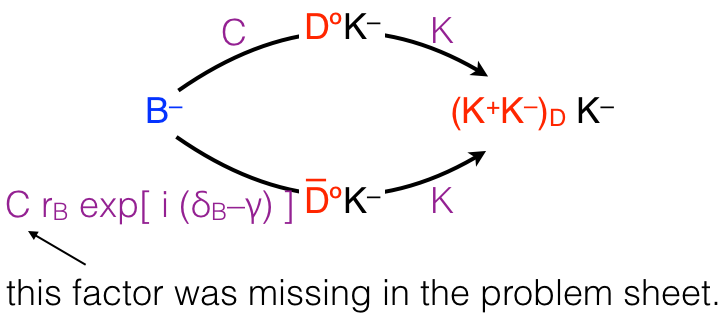
\includegraphics[width=0.5\textwidth]{problemsheets/ps2figs/B2DK_D2KK_interference_labelled}\\
 (This has no purpose other than visualising and organising what goes on, which can be helpful in the subsequent calculations.)
 \item If you apply the \cp\ operation to this amplitude ratio, you get:
  \[
    \frac{A(\prt{B^+ \to \Do K^+})}{\prt{A(B^+ \to \Dob K^+})} = r_B e^{i(\delta_B + \gamma)}
 \]
 Explain why.
 \answerbox{The strong interaction respects \cp\ symmetry, so all factors introduced by it (including the phase $\delta_B$) remain invariant. For the weak interaction, the \cp\ operation has the effect of complex conjugating the CKM matrix element, so we take the negative of all phases introduced by the CKM matrix, here: $\gamma \to -\gamma$. The magnitudes remain the same, so:
 $
 \left|\frac{A(\prt{B^- \to \Dob K^-})}{\prt{A(B^- \to \Do K^-})} \right| = 
 \left|\frac{A(\prt{B^+ \to \Do K^+})}{\prt{A(B^+ \to \Dob K^+})} \right|
 $
 and hence, the effect of \cp\ is: $r_B \to r_B$, $\delta_B \to \delta_B$, $\gamma \to -\gamma$.
 }
 \item Calculate the rate asymmetry
 \[
  A = \frac{ 
    \Gamma(B^- \to (K^+ K^-)_D K^-) -
    \Gamma(B^+ \to (K^+ K^-)_D K^+)
  }{ 
    \Gamma(B^- \to (K^+ K^-)_D K^-) +
    \Gamma(B^+ \to (K^+ K^-)_D K^+)
  }
 \]
 in terms of $r_B$, $\delta_B$, $\gamma$ (the $C$ and $K$ will cancel, if you want you can simply set them to $1$ straight from the beginning).
 \end{itemize}
 \answerbox{
     \begin{eqnarray*}
      \Gamma(B^-) & = & 
      \left| CK + CK r_B e^{i(-\gamma + \delta_B)} \right|^2
      \\ & = &
      C^2 K^2 \left(1 + r_B^2 + 2\,r_B\,\cos\left(-\gamma +\delta_B \right)\right)
      \\ & = & C^2K^2\left(1 + r_B^2 + 2\,r_B\, \left(
        \cos(\delta_B)\,\cos\gamma {\color{red} +} 
        \sin(\delta_B)\,\sin\gamma\right)\right)
      \\ \Gamma(B^+) & = & 
      \left| CK + CK r_B e^{i(+\gamma + \delta_B)} \right|^2
      \\ & = &
      C^2 K^2 \left(1 + r_B^2 + 2 r_B\,\cos\left(+\gamma +\delta_B \right)\right)
      \\ & = & C^2 K^2 \left(1 + r_B^2 + 2 r_B\, \left(
        \cos(\delta_B)\,\cos\gamma {\color{red} -}
          \sin(\delta_B)\,\sin\gamma\right)\right)
      \\ A_{CP}^{KK} & = & 
      \frac{
        2 r_B\,\sin(\delta_B)\,\sin\gamma
      }{
        1 + r_B^2 + r_B\, \cos(\delta_B)\,\cos\gamma
      } 
    \end{eqnarray*}
    }   
    \item Repeat the calculation for
  \[
  A = \frac{ 
    \Gamma(B^- \to (K^+ \pi^-)_D K^-) -
    \Gamma(B^+ \to (K^- \pi^+)_D K^+)
  }{ 
    \Gamma(B^- \to (K^+ \pi^-)_D K^-) +
    \Gamma(B^+ \to (K^- \pi^+)_D K^+)
  }
 \]
 Note that there will additional parameters because the ratio of the \Do, \Dob\ decay amplitudes does not cancel as in the case above, but instead:
  \[
    \frac{A(\prt{\Do \to K^+ \pi^-})}{A(\prt{\Dob\to K^+\pi^-})} = r_D^{K\pi} e^{i\delta_D}
 \]
 \answerbox{
    In the previous part, with used
    $\frac{A(\prt{\Do \to K^+ K-})}{A(\prt{\Dob\to K^+K-})}=1$, which is fundamentally because there is no \cp\ violation in \Do\ decays, and the final state is a \cp\ eigenstate. We could also have arrived at this result by drawing the Feynman diagrams for both decays, using the appropriate CKM matrix elements (and that the CKM matrix elements involved in \Do\ decays are all real is ultimately the reason that there is no \cpv\ in \Do\ decays).
     
    Now that the \Do, \Dob\ do not decay to a \cp\ eigenstate anymore we actually need to take into account that 
    \[
    \frac{A(\prt{\Do \to K^+ \pi^-})}{A(\prt{\Dob\to K^+\pi^-})} = r_D^{K\pi}  e^{i\delta_D}
    \]
    Note that there is no weak phase that would change under \cp. You can get this by drawing diagrams, or just remember that there is no \cpv\ in D meson decays. So $\delta_D$ is the strong phase difference between the \Do\ and \Dob\ decay amplitude to $\Kp\pim$.
    
    Our interference sketch looks now like this:
    \\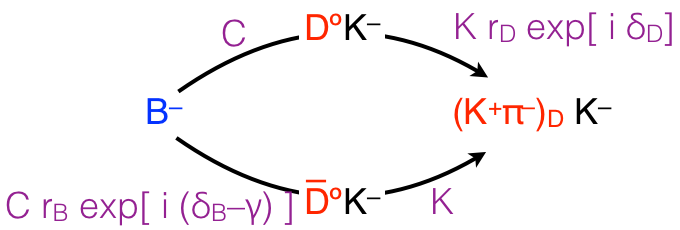
\includegraphics[width=0.5\textwidth]{problemsheets/ps2figs/B2DK_D2Kpi_Interference}\\
    
     \begin{eqnarray*}
      \Gamma(B^-) & = & 
      \left| CK r_D^{K\pi} e^{i\delta_D^{K\pi}} + CK r_B e^{i(-\gamma + \delta_B)} \right|^2
      \\ & = &
      C^2 K^2 \left({r_D^{K\pi}}^2 + r_B^2 + 2r_D^{K\pi}\,r_B\,\cos\left(-\gamma +\delta_B-\delta_D^{K\pi} \right)\right)
      \\ & = & C^2K^2\left({r_D^{K\pi}}^2 + r_B^2 + 2r_D^{K\pi}\,r_B\, \left(
        \cos(\delta_B-\delta_D^{K\pi})\,\cos\gamma {\color{red} +}
        \sin(\delta_B-\delta_D^{K\pi})\,\sin\gamma\right)\right)
      \\ \Gamma(B^+) & = & 
      \left| CK r_D^{K\pi} e^{i\delta_D^{K\pi}} + CK r_B e^{i(+\gamma + \delta_B)} \right|^2
      \\ & = &
      C^2 K^2 \left({r_D^{K\pi}}^2 + r_B^2 + 2r_D^{K\pi}\,r_B\,\cos\left(+\gamma +\delta_B-\delta_D^{K\pi} \right)\right)
      \\ & = & C^2 K^2 \left({r_D^{K\pi}}^2 + r_B^2 + 2r_D^{K\pi}\,r_B\, \left(
        \cos(\delta_B -\delta_D^{K\pi})\,\cos\gamma 
        {\color{red} -} \sin(\delta_B-\delta_D^{K\pi})\,\sin\gamma\right)\right)
      \\ A_{CP}^{K\pi} & = & 
      \frac{
        2r_D^{K\pi}\,r_B\,\sin(\delta_B-\delta_D^{K\pi})\,\sin\gamma
      }{
        {r_D^{K\pi}}^2 + r_B^2 + 2r_D^{K\pi}\,r_B\, \cos(\delta_B-\delta_D^{K\pi})\,\cos\gamma
      } 
      \\ & = & 
      \frac{
        2\,\frac{r_B}{r_D^{K\pi}}\,\sin(\delta_B-\delta_D^{K\pi})\,\sin\gamma
      }{
        1 + \left(\frac{r_B}{r_D^{K\pi}}\right)^2 
        + 2\frac{r_B}{r_D^{K\pi}} \cos(\delta_B-\delta_D^{K\pi})\,\cos\gamma
      } 
      \\ & & \mbox{which is the same as}
        \\ & = & 
      \frac{
        2\,\frac{r_D^{K\pi}}{r_B}\,\sin(\delta_B-\delta_D^{K\pi})\,\sin\gamma
      }{
        1 + \left(\frac{r_D^{K\pi}}{r_B}\right)^2 
        + 2\frac{r_D^{K\pi}}{r_B} \cos(\delta_B-\delta_D^{K\pi})\,\cos\gamma
      } 
    \end{eqnarray*}
 }
 \item Which of the two asymmetries is larger? Estimate an approximate numerical value.
 \answerbox{The difference between the two asymmetries is that, to get from $A_{CP}^{KK}$ to $A_{CP}^{K\pi}$,  we need to replace $r_B$ with $r_B/r_D^{K\pi}$, or, equivalently with $r_D^{K\pi}/r_B$. The best sensitivity is reached for when this factor is $\sim 1$, to the question comes down to whether $r_B$ or $r_D^{K\pi}/r_B$ is closer to $1$ (note
 
 So let's estimate $r_D$. The relevant Feynman diagrams are:
 \\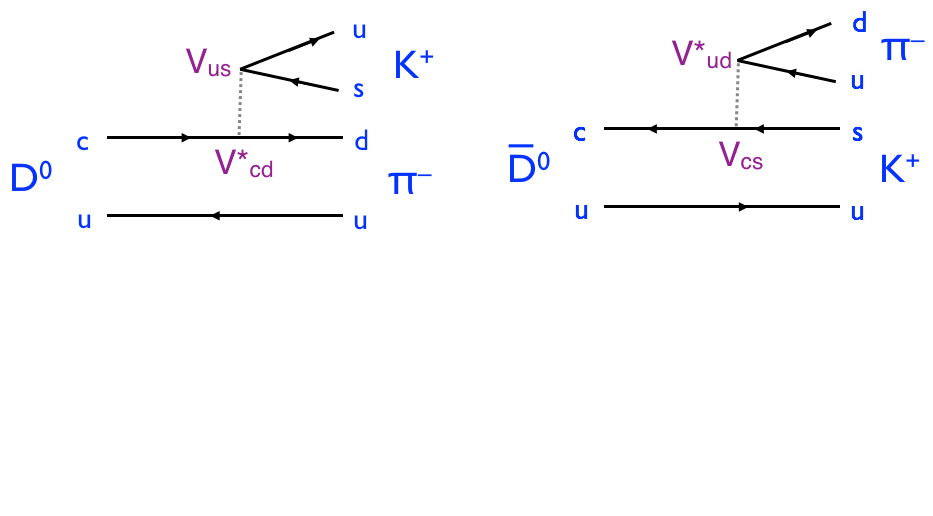
\includegraphics[width=0.65\textwidth]{problemsheets/ps2figs/D2KpiDiagrams}.\\
 Multiplying the relevant CKM matrix elements:
    \[
     \frac{A(\prt{\Do \to K^+ \pi^-})}{A(\prt{\Dob\to K^+\pi^-})}
     =
     \frac{V_{cd}^* V_{us}}{ V_{ud}^* V_{cs}}
     \approx \cos^2(\theta_C) = 0.05
    \]
 So, we estimate $r_D/r_B \sim 0.25$. It turns out that the measured values for $r_B$ is $0.01$, somewhat smaller than our estimate, while our estimate for $r_D$ is spot-on, so really, $r_D/r_B \sim 0.5$.
 
 To estimate the size of the asymmetry, we need to know $\delta_B$ and $\delta_D$. We cannot calculate those, but we can get an estimate of the maximum value that the asymetries can obtain by assuming they are such that the cosine of the strong phase differences is $0$ and the sine is $1$, leading to
 \begin{eqnarray*}
     A_{CP}^{KK} 
       & \leq & 
      \frac{
        2\,r_B\,\sin\gamma
      }{
        1 + r_B^2 
      }
  \\ A_{CP}^{K\pi} 
       & \leq & 
      \frac{
        2\,\frac{r_D^{K\pi}}{r_B}\,\sin\gamma
      }{
        1 + \left(\frac{r_D^{K\pi}}{r_B}\right)^2 
      } 
  \end{eqnarray*}
 Putting in the values we calculated in this exercise, we get
  \begin{eqnarray*}
     A_{CP}^{KK} 
       & \leq & 
      \frac{
        2 \cdot 0.22 \sin(68^{\circ})
      }{
        1 + 0.22^2 
      } = 0.38
  \\ A_{CP}^{K\pi} 
       & \leq & 
      \frac{
        2\cdot 0.25\,\sin(68^{\circ})
      }{
        1 + 0.25^2 
      } =0.48
  \end{eqnarray*}
 These are both quite large numbers (\cp\ assymetries of about 40-50\%, that's a big effect). Using the measured value of $r_B$ instead, we get
  \begin{eqnarray*}
     A_{CP}^{KK} 
       & \leq & 
      \frac{
        2 \cdot 0.1 \sin(68^{\circ})
      }{
        1 + 0.1^2 
      } = 0.18
  \\ A_{CP}^{K\pi} 
       & \leq & 
      \frac{
        2\cdot 0.5\,\sin(68^{\circ})
      }{
        1 + 0.5^2 
      } =0.74
  \end{eqnarray*}
 Now the difference between the two methods becomes much clearer. While $A_{CP}^{KK}$ can go up to $18\%$, $A_{CP}^{K\pi}$ could be as large as $74\%$!! \cp\ violation in the B hadrons is indeed not a small effect.
 }
\end{enumerate}

 

\subsection{Summary of \cpv\ phenomenology}
\begin{itemize}
\item There are three types of \cpv: \cpv\ in mixing, \cpv\ in decay, and \cpv\ in the interference between mixing and decay.
\item \cpv\ in mixing is the dominant \cp--violating effect in the Kaon system, while in the B system, it is negligible. The mechanisms of \cpv\ in B hadrons is direct \cpv\ and \cpv\ in the interference between mixing and decay.
\item \cpv\ is an interference effect, and needs therefore at least two interfering decay amplitudes.
\item \cpv\ can be very large in B-hadron decays, because it will involve, even at tree-level, all three generations (while in kaon decays, the 3rd generation only enters indirectly through loops). B hadrons give us access to the ony two CKM matrix element with large complex phases, $V_{td}$ (which enters in \Bdo\ mixing, usually measured time-dependent decay rate asymmetries) and $V_{ub}$ (in all decays involving $b \to u$ transitions).
\item We learnt how to calculate \cp-violating asymmetries in decays such as \prt{\Bm \to (K^+\pi^-)_D\Km} and its \cp-conjugate, and in \prt{\Bm \to (K^+K^-)_D\Km} and its \cp-conjugate.
\item We learnt how to calculate the amplitude of time-dependent decay rate asymmetries in \cp\ violation measurements in neutral B meson decays to \cp\ eigenstates like \prt{\Bdo \to J/\psi K_S}. It's the sine of the phase difference of the interfering decay paths.
\end{itemize}

